\section{Experimental Evaluation} \label{sec:experimental_evaluation}

In this section, the experiments and results are presented. First, the datasets used to conduct the experiments and test the crest-line detection methods is presented in section \ref{subsec:study-areas}. Two main datasets were used for the study:

\begin{description}[align=left]
	\item[Terrestrial Dataset] A sample dataset of various regions created and labeled by an expert in the field, specifically for this research.
	\item[Mars Dataset] The dataset from the Ganges Crater area on Mars, defined by \cite{vaz_object_based_dune_analysis}.
\end{description}

The next section discusses the evaluation used for measuring the quality of each dune crest-line detector method. The main metrics used are the Precision, Recall, and dune features presented in section \ref{subsec:dune_field_metrics}. Finally, section \ref{subsec:results-and-discussion} presents the results along with a short discussion of the methods. 

\subsection{Study Areas} \label{subsec:study-areas}

As part of this research project, two datasets were used in order to evaluate the robustness of each method. The datasets include a wide range of dune types with varying morphological properties. The data provided in each set are satellite images of dune field regions available through Google Earth and NASA datasets. Included with the images is the ground truth which has been manually labeled by experts in the research field. The ground truth consists of crest-lines for each positive dune detection. In each case, the scales of the satellite images were chosen such that the inter-dune distance appeared roughly normalized across the entire dataset. Scale selection of the images is important process for even comparison of the methods for different regions. The images are resized to an appropriate resolution for processing and even across the entire dataset.

The method described in this paper was tested on two distinct datasets: an terrestrial dataset which includes dune fields of various regions on Earth, along with the dataset provided in \cite{vaz_object_based_dune_analysis} which is located on Mars in the Ganges crater region. The same method was applied on both datasets.

\subsubsection{Terrestrial Dataset}
\label{subsec:terrestrial_dataset}
The first dataset is a small sample of a dozen satellite images from six separate desert regions on Earth (shown in Figure \ref{fig:terrestrial_dataset}). Included are the Kalahari, Namib and Skeleton Coast sand sea regions in Namibia (\cite{goudie_desert_landforms_namibia}). Also represented in this dataset are the Simpson dune field in Australia, the Winnemucca Dune Complex in Nevada, and the White Sands National Monument. A wide range of landforms types are contained within each of these regions which provides a broad study for an automated crest-line detection method. 

\begin{figure*}[htbp]
	\centering
	\begin{subfigure}[b]{0.3\textwidth}
		\centering
		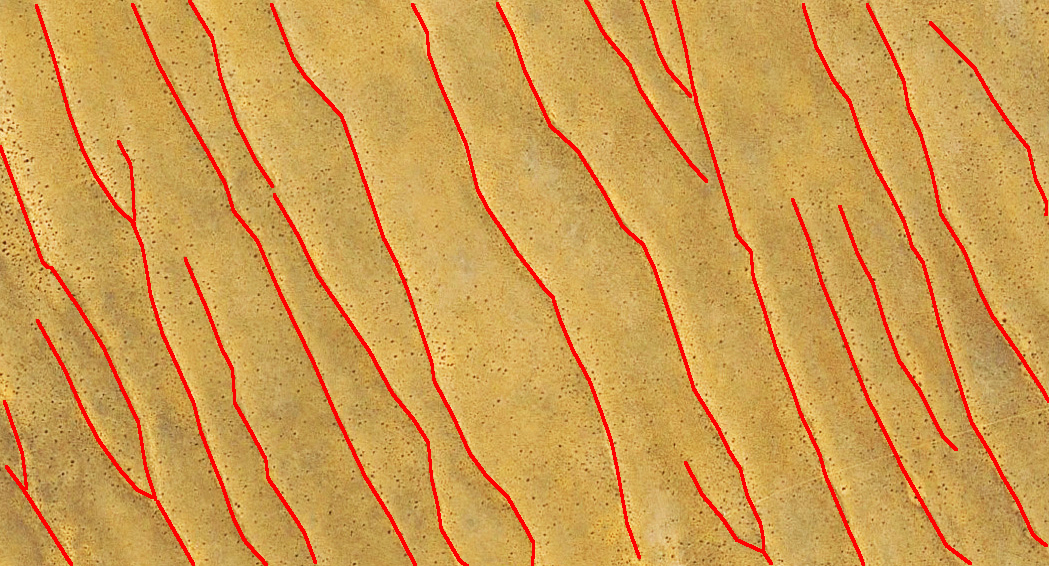
\includegraphics[width=\textwidth]{figures/kalahari_with_gt}
		\caption{ Kalahari }
	
		\label{fig:kalahari_image}
	\end{subfigure}
	\begin{subfigure}[b]{0.3\textwidth}
		\centering	
		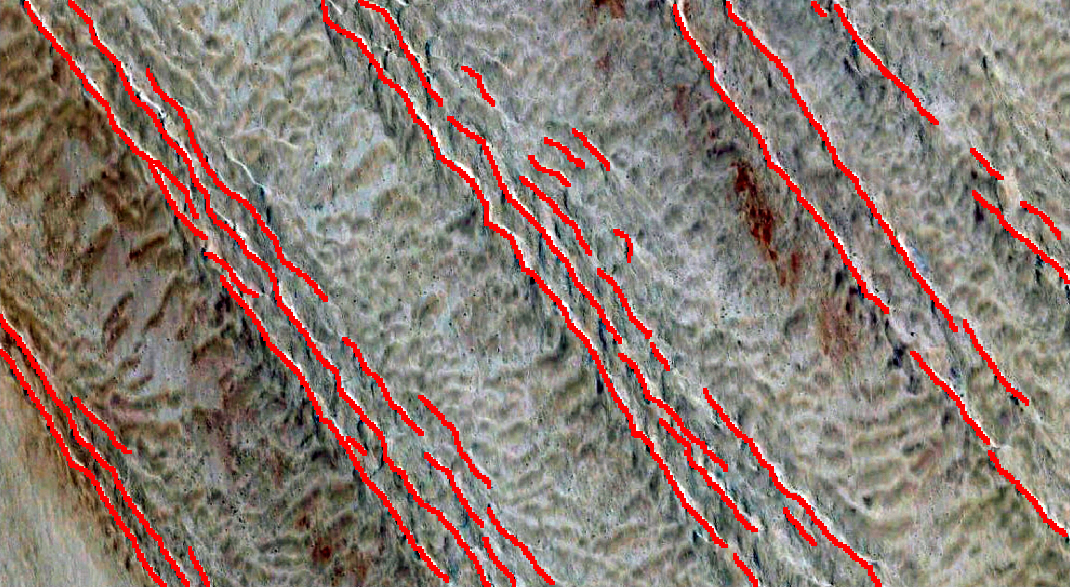
\includegraphics[width=\textwidth]{figures/namib_with_gt}
		\caption{ Namib }
		\label{fig:namib_image}
	\end{subfigure}
	\begin{subfigure}[b]{0.3\textwidth}
		\centering
		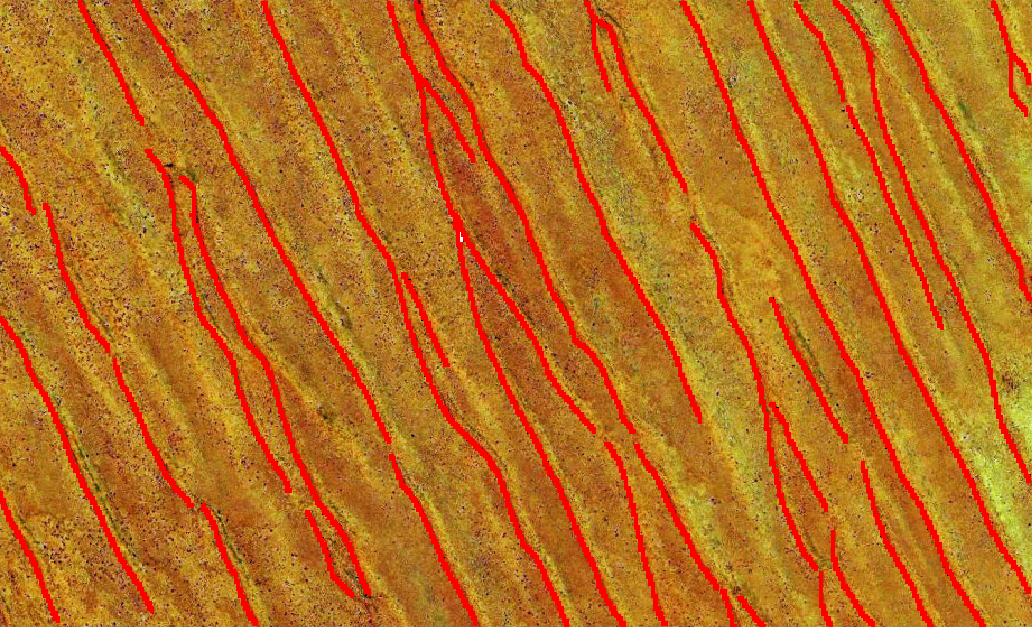
\includegraphics[width=\textwidth]{figures/simpson_with_gt}
		\caption{ Simpson }
		\label{fig:simpson_image}
	\end{subfigure}
	\begin{subfigure}[b]{0.3\textwidth}
		\centering
		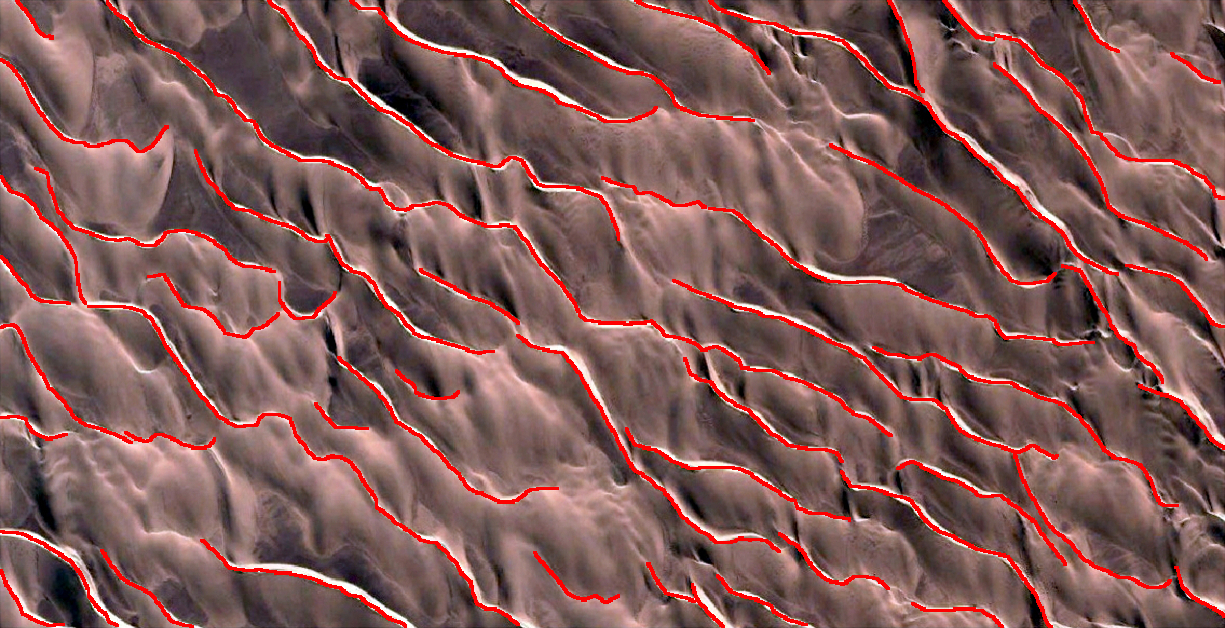
\includegraphics[width=\textwidth]{figures/skeleton_coast_with_gt}
		\caption{ Skeleton Coast }
		\label{fig:skeleton_coast_image}
	\end{subfigure}
	\begin{subfigure}[b]{0.3\textwidth}
		\centering
		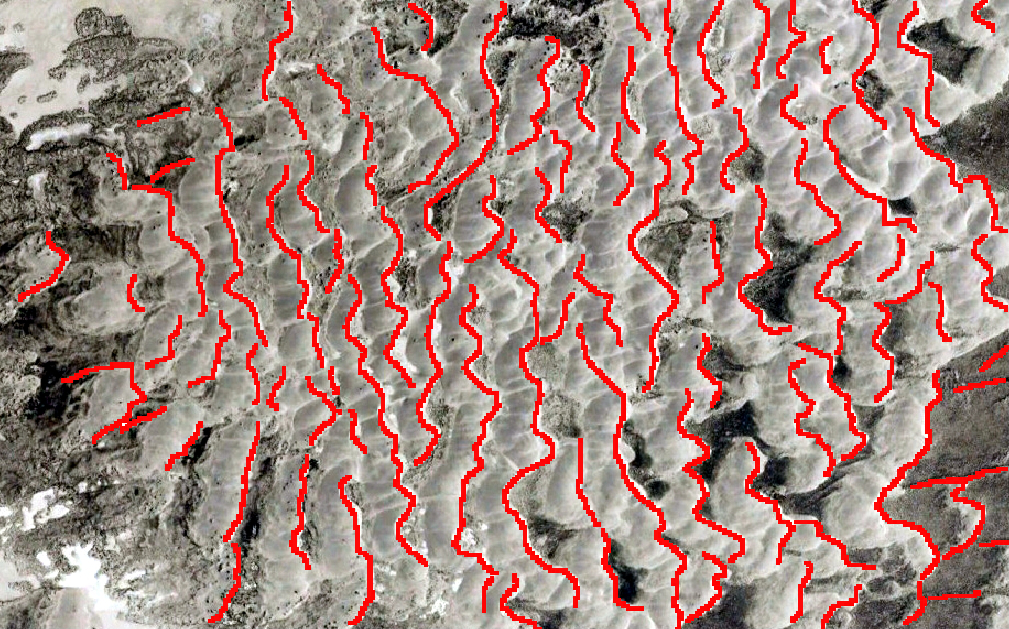
\includegraphics[width=\textwidth]{figures/wdc_with_gt}
		\caption{  Winnemucca Dune Complex }
		\label{fig:wdc_image}
	\end{subfigure}
	\begin{subfigure}[b]{0.3\textwidth}
		\centering
		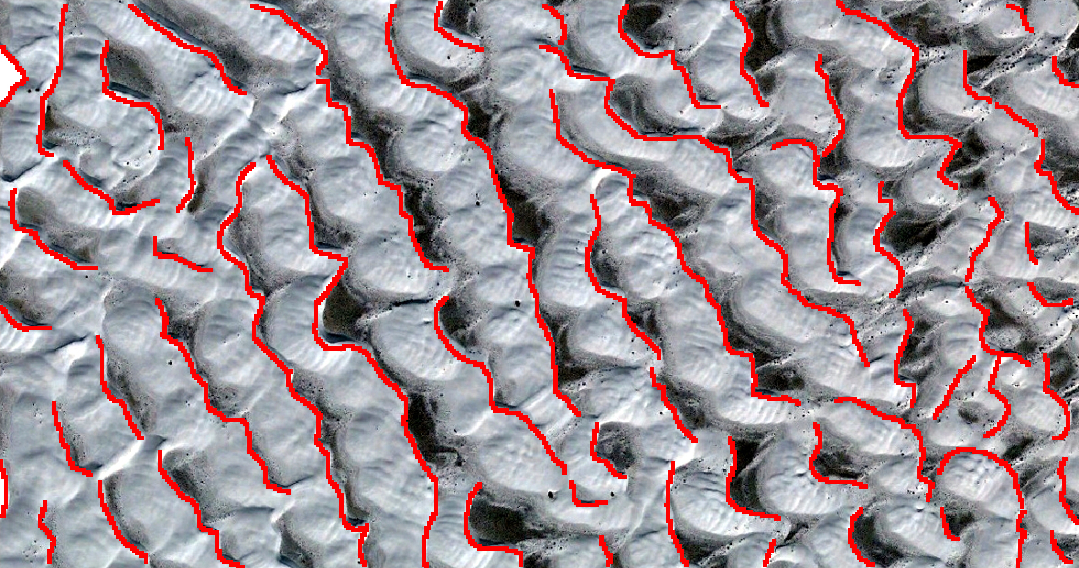
\includegraphics[width=\textwidth]{figures/whitesands_with_gt}
		\caption{ White Sands }
		\label{fig:white_sands_image}
	\end{subfigure}
	\caption{Terrestrial dataset of six regions with respective labeled ground truth: (\ref{fig:kalahari_image}) Kalahari (Namibia), (\ref{fig:namib_image}) Namib (Namibia), (\ref{fig:simpson_image}) Simpson (Australia), (\ref{fig:skeleton_coast_image}) Skeleton Coast (Namibia), (\ref{fig:wdc_image}) Winnemucca Dune Complex (USA), and (\ref{fig:white_sands_image}) White Sands (USA)}
	\label{fig:terrestrial_dataset}
\end{figure*}

The Kalahari (Figure \ref{fig:kalahari_image})sands span from the southeastern region of Namibia to South Africa. The region is a 100-200 km wide and is composed of mostly fixed dunes \cite{lancaster_linear_dunes_kalahari}. Most of the area is comprised of simple linear form dunes, although some small areas contain some compound linear dunes as well. Unlike other desert regions, the Kalahari contains areas which are well vegetated. On average, the dunes range from 2m to 15m in height, with a 150m to 250m width, and spaced from 200m to 240m. These measurements may be useful for determining the reliability of our metric calculations.

The Namib Sand Sea (Figure \ref{fig:namib_image}) region spans approximately 34,000 km of the Altantic coast of Namibia, contains some of the largest and oldest sand dunes in the world according to \cite{goodie_namib_sand_sea_ancient_desert}. High energy unimodal, bimodal and complex wind regimes create interesting dune field patterns in the Namib Sand Sea region of Namibia \cite{lancaster_winds_sand_movement_namib_sea}. These wind patterns characterize the spatial variability of the dune types, sizes, and other morphological properties of the region, making it an interesting case study for this research.

The Skeleton Coast (Figure \ref{fig:skeleton_coast_image}) dune field contains simple, locally compound, transverse and barchanoid dunes over its 2000 km\textsuperscript{2} span according to \cite{lancaster_dunes_skeleton_coast}. The dunes pattern in this region are formed due to onshore winds and surface roughness changes between the dunes and coastal plains. The dune field is roughly aligned with the coast and is characterized with a large slip face in which dunes range from 20m to 80m in height.

Another region represented in the dataset is the Simpson (Figure \ref{fig:simpson_image}) dune field in Australia. Much like the Kalahari sands in southern Africa, the Simpson dune fields contains many similar features. The areas are home to lush vegetation, and the dune field follow a mostly simple linear pattern where the dunes tend to be broad crested \cite{hesse_australian_desert_dunefields}. According to \cite{twidale_simpson_desert_australia}, some of the ridges continue unbroken for up to 200 km, where each crest measures 15m to 38m in height. The spacing between each crest varies depending on the height of the ridges. Areas with larger ridges may have one or two dunes per kilometer, while smaller ridges may have five or six dunes per kilometer. These factor make this area an interesting addition to the dataset because the scale of the images is much larger.

Also present is the Winnemucca Dune Complex (WDC, Figure \ref{fig:wdc_image}) found in the western United States, in Nevada. The WDC covers an area of roughly 900 km\textsuperscript{2} north of Winnemucca, Nevada. The most common dune type present are stabilized parabolic dunes, but barchans and transverse ridges can also be found scattered throughout the area \cite{zimbelman_eolian_deposits_western_united_states}. In fact, according to \cite{pepe_winnemucca_dune_complex}, the WDC is primarily covered by six crescentic complexes, a large sand sheet, and discontinuous sets of compound barchanbolic-parabolic dune fields. The WDC contains a complex set of repetitive sequences of dunes which varying shapes and scales, which makes it an ideal candidate for this dataset.

Finally, the last area in the dataset is the White Sands National Monument (fig. \ref{fig:white_sands_image}), located in the state of New Mexico, USA. This area boasts an interesting pattern of crescentric aeolian dunes which are formed in a systematically similar fashion to wind ripples and sub-aqueous dunes \cite{ewing_aeolian_dune_interaction_white_sands}. There are a wide range of features and properties in the White Sands dune field that merit study, such as described in \cite{ewing_aeolian_dune_interaction_white_sands}. These interactions include merging, lateral linking, defect repulsion, bed-form repulsion, off-center collision, defect creation and dune splitting. The details of these interactions are outside the scope of this research but crest-line detection may be an essential preliminary step towards extracting those features. Measuring the number of dunes, crest lengths, defect density, dune spacing, and dune height are all done manually by experts in the field. A move towards an automated process would greatly improve research efforts, and would be a helpful tool for scientist in the field.

\subsubsection{Mars Dataset}
\label{subsec:mars_dataset}
To verify the robustness of this approach, the method was also tested on another dataset which was used in \cite{vaz_object_based_dune_analysis}. The dataset provided is from the Ganges Chasms on Mars, and includes satellite images, manually labeled crest-lines, and the results of the original author's method. The provided results lay a baseline benchmark for measuring quality and accuracy of crest-line detection algorithms. In order to more easily process the dataset, the Ganges region was split into sixteen areas of equal size, as shown in Figure \ref{fig:mars_ganges_dataset}. The ground truth included was not validated for correctness, the labeled data was used as-is, which may account for some errors (see Section \ref{subsec:results-and-discussion}).

\begin{figure*}[htbp]
	\centering
	\begin{subfigure}[b]{0.3\textwidth}
		\centering
		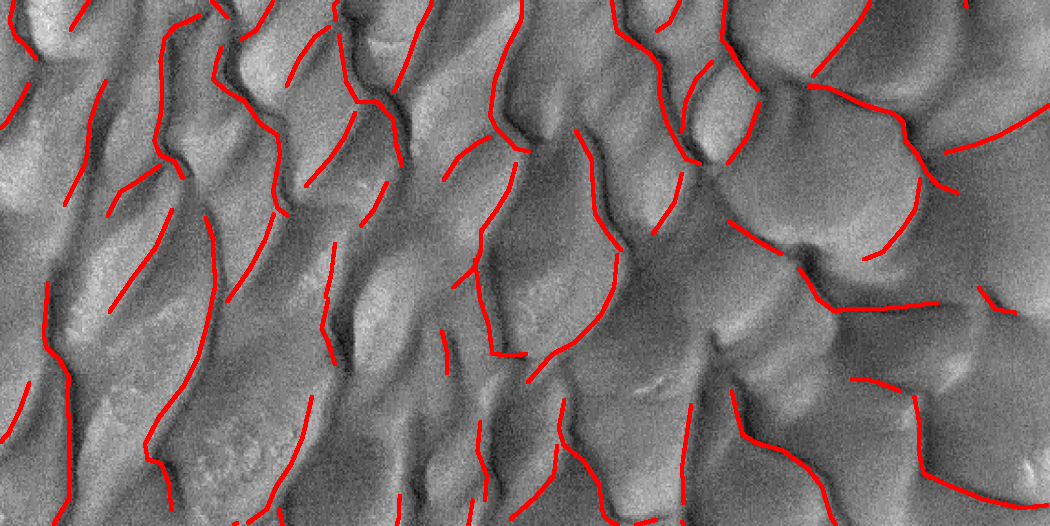
\includegraphics[width=\textwidth]{figures/area1_with_gt}
		\caption{  Region 1 }
		\label{fig:area1_image}
	\end{subfigure}
	\begin{subfigure}[b]{0.3\textwidth}
		\centering	
		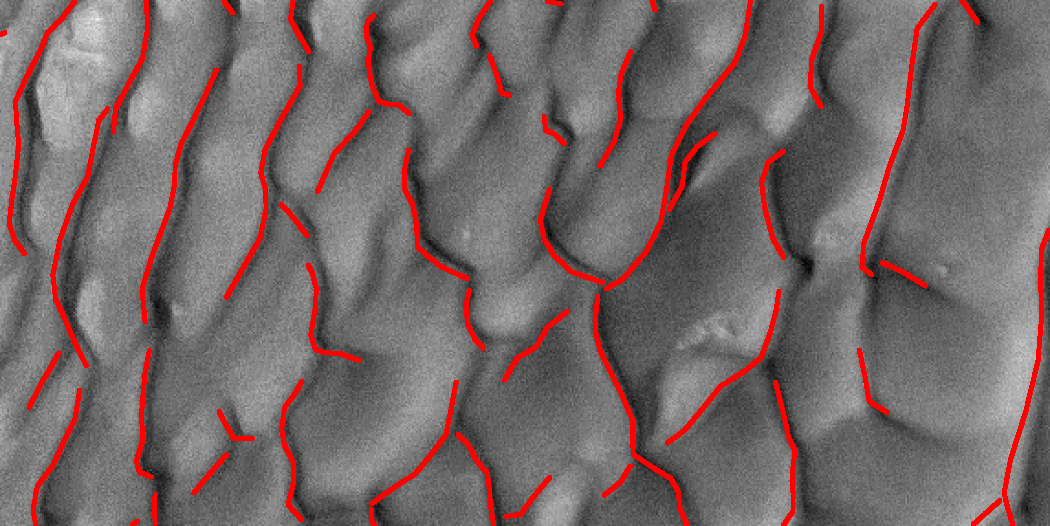
\includegraphics[width=\textwidth]{figures/area2_with_gt}
		\caption{  Region 2 }
		\label{fig:area2_image}
	\end{subfigure}
	\begin{subfigure}[b]{0.3\textwidth}
		\centering
		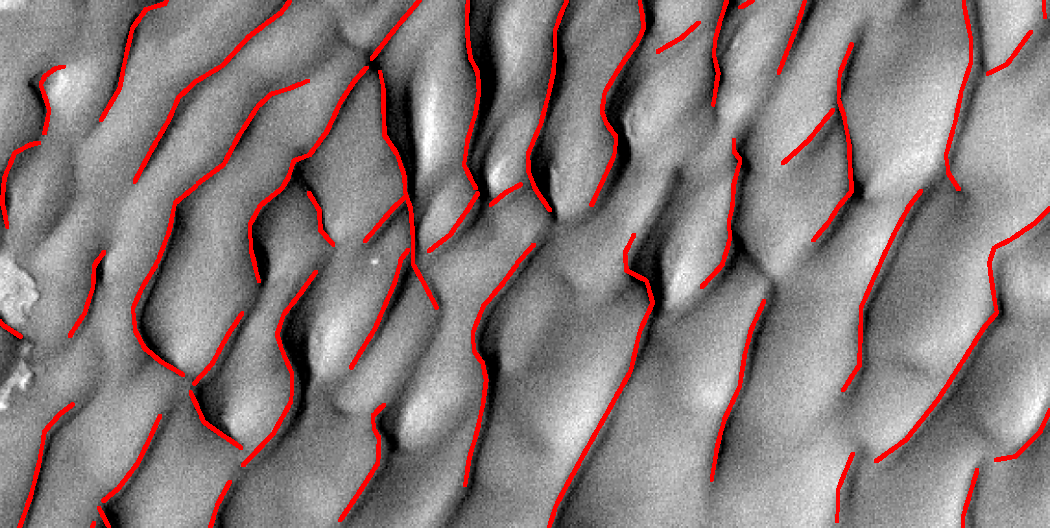
\includegraphics[width=\textwidth]{figures/area3_with_gt}
		\caption{  Region 3 }
		\label{fig:area3_image}
	\end{subfigure}
	\begin{subfigure}[b]{0.3\textwidth}
		\centering
		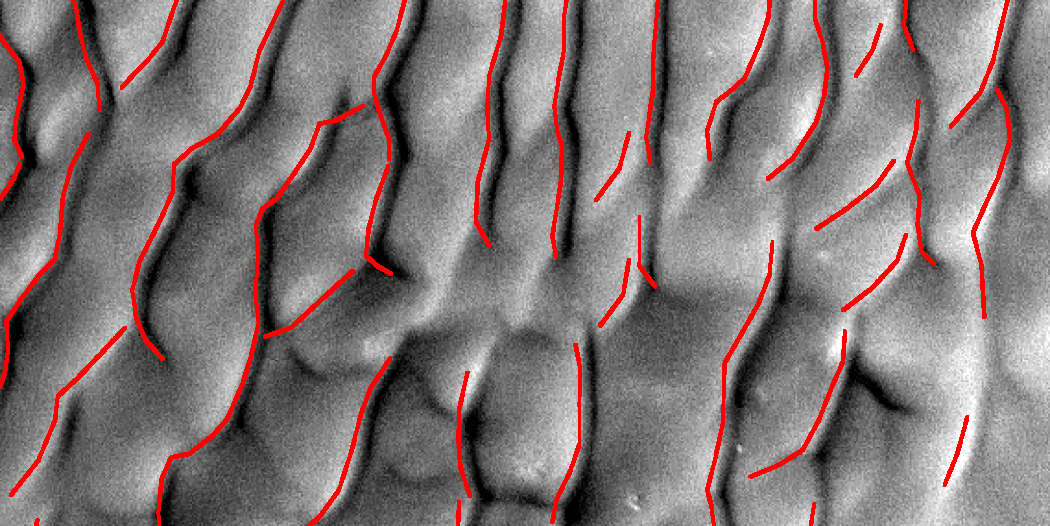
\includegraphics[width=\textwidth]{figures/area4_with_gt}
		\caption{  Region 4 }
		\label{fig:area4_image}
	\end{subfigure}
	\begin{subfigure}[b]{0.3\textwidth}
		\centering
		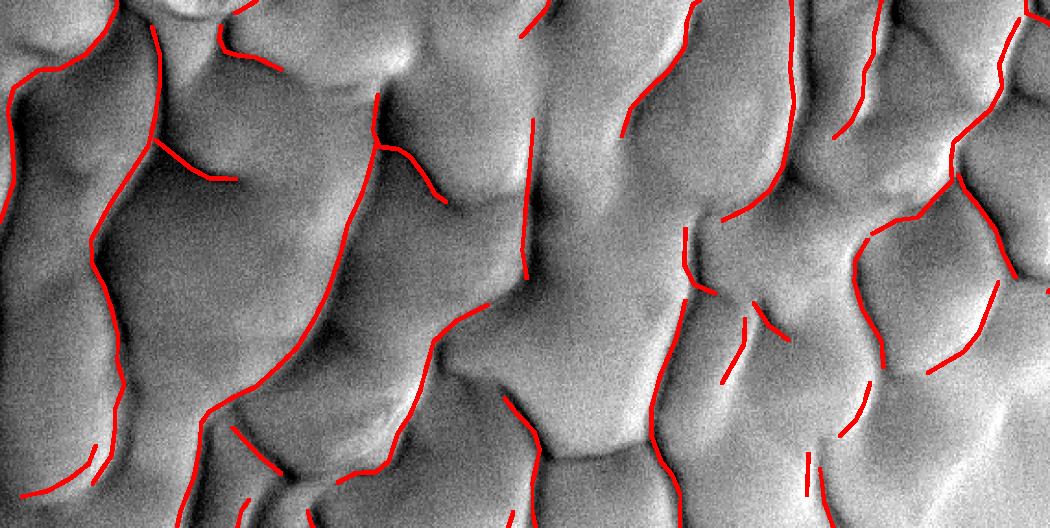
\includegraphics[width=\textwidth]{figures/area5_with_gt}
		\caption{  Region 5 }
		\label{fig:area5_image}
	\end{subfigure}
	\begin{subfigure}[b]{0.3\textwidth}
		\centering
		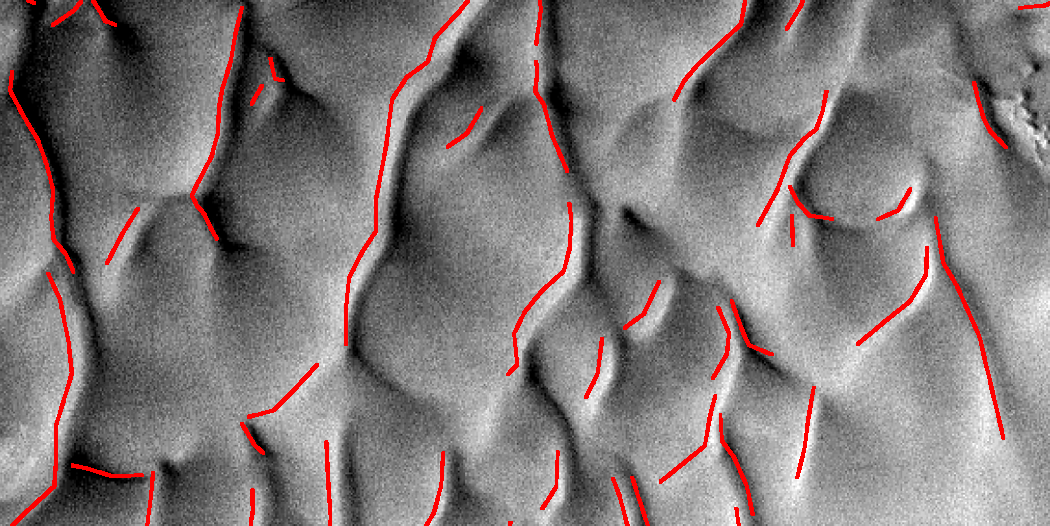
\includegraphics[width=\textwidth]{figures/area6_with_gt}
		\caption{  Region 6 }
		\label{fig:area6_image}
	\end{subfigure}
	\begin{subfigure}[b]{0.3\textwidth}
		\centering
		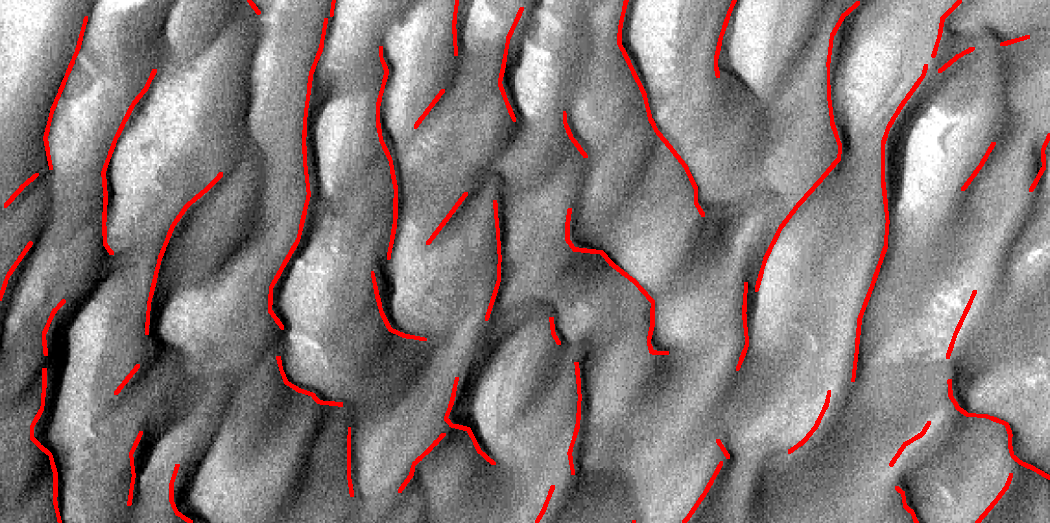
\includegraphics[width=\textwidth]{figures/area7_with_gt}
		\caption{  Region 7 }
		\label{fig:area7_image}
	\end{subfigure}
	\begin{subfigure}[b]{0.3\textwidth}
		\centering
		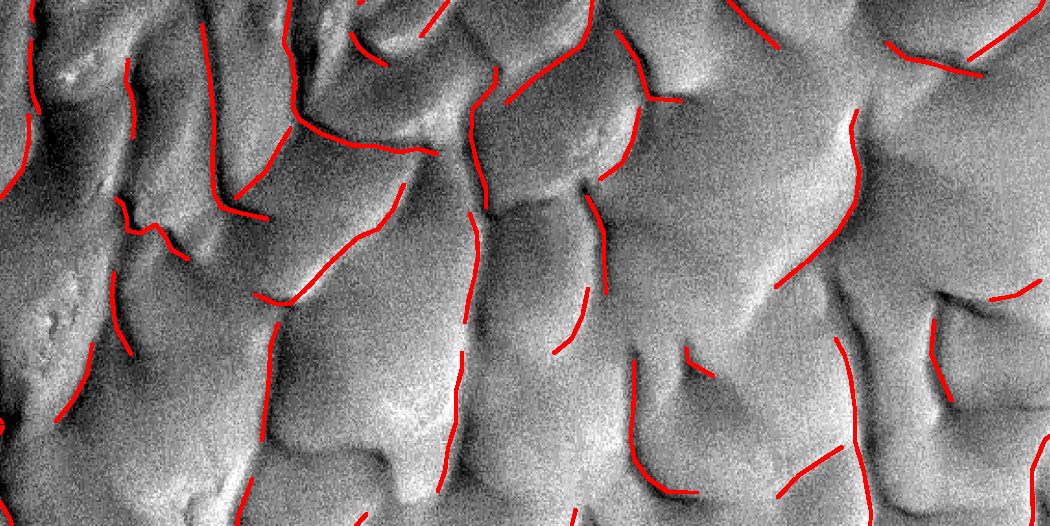
\includegraphics[width=\textwidth]{figures/area8_with_gt}
		\caption{  Region 8 }
		\label{fig:area8_image}
	\end{subfigure}
	\begin{subfigure}[b]{0.3\textwidth}
		\centering
		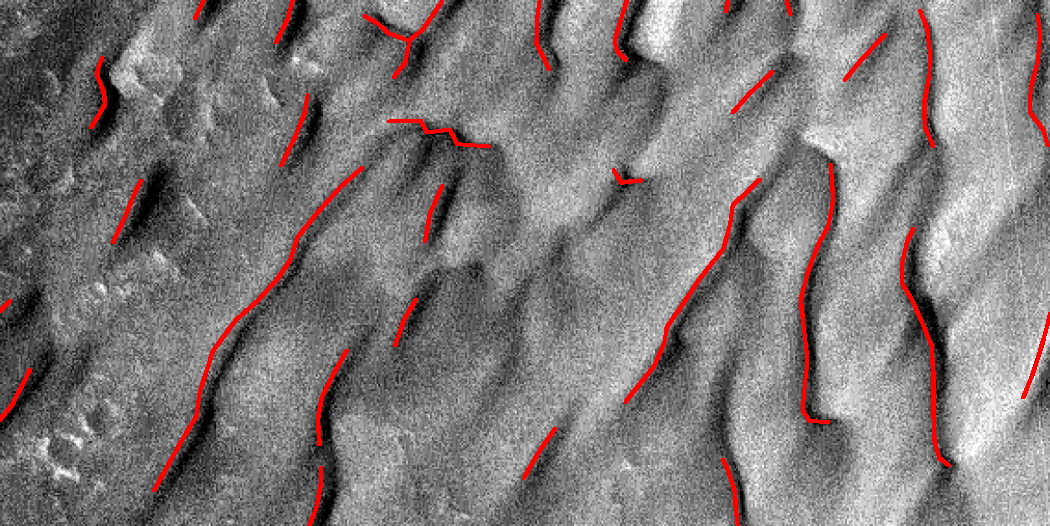
\includegraphics[width=\textwidth]{figures/area9_with_gt}
		\caption{  Region 9 }
		\label{fig:area9_image}
	\end{subfigure}

	\begin{subfigure}[b]{0.3\textwidth}
		\centering
		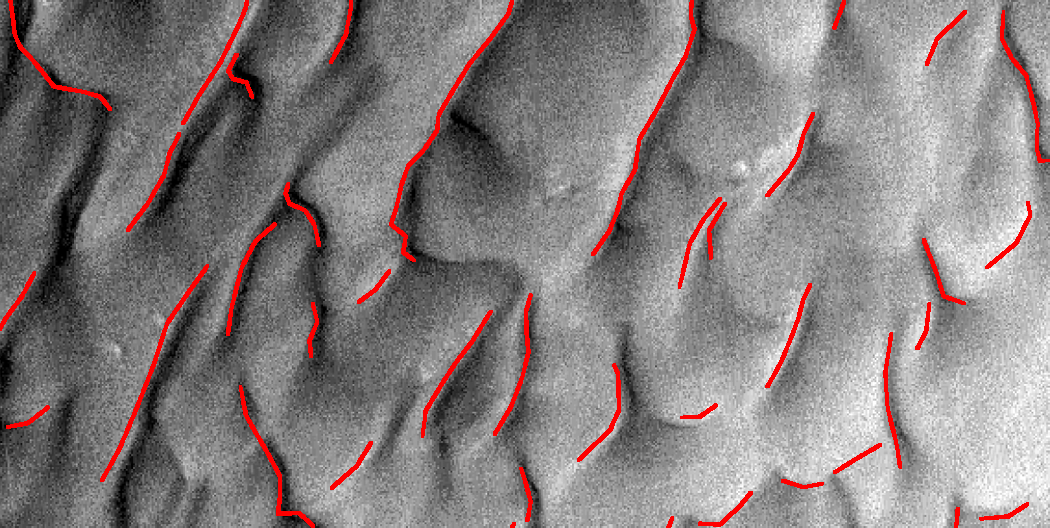
\includegraphics[width=\textwidth]{figures/area10_with_gt}
		\caption{  Region 10 }
		\label{fig:area10_image}
	\end{subfigure}
	\begin{subfigure}[b]{0.3\textwidth}
		\centering
		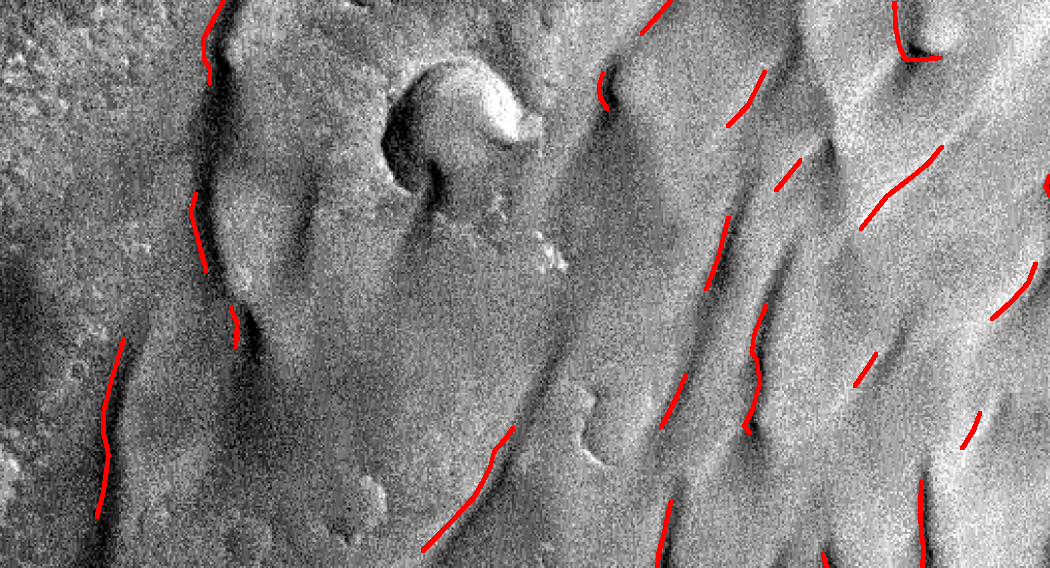
\includegraphics[width=\textwidth]{figures/area11_with_gt}
		\caption{  Region 11 }
		\label{fig:area11_image}
	\end{subfigure}
	\begin{subfigure}[b]{0.3\textwidth}
		\centering
		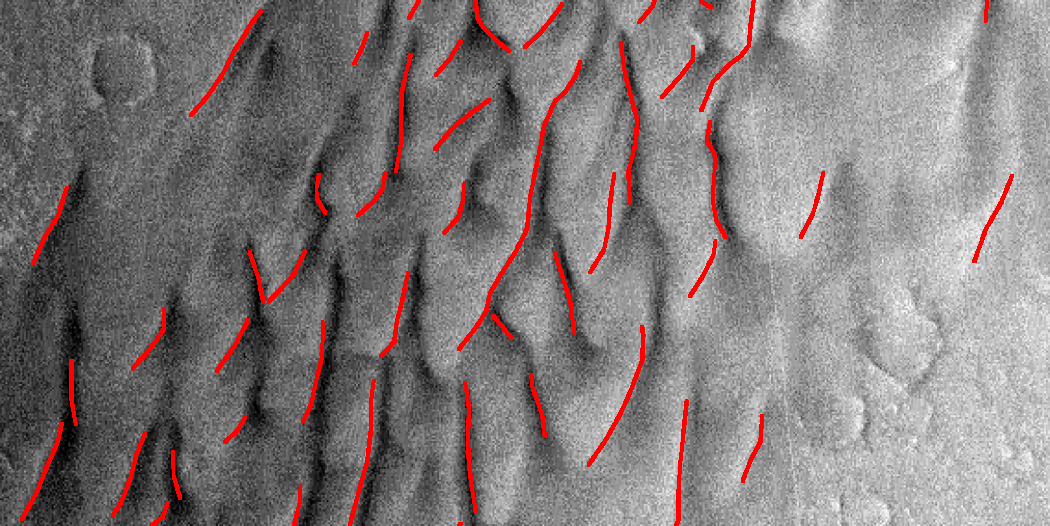
\includegraphics[width=\textwidth]{figures/area12_with_gt}
		\caption{  Region 12 }
		\label{fig:area12_image}
	\end{subfigure}
	\begin{subfigure}[b]{0.3\textwidth}
		\centering
		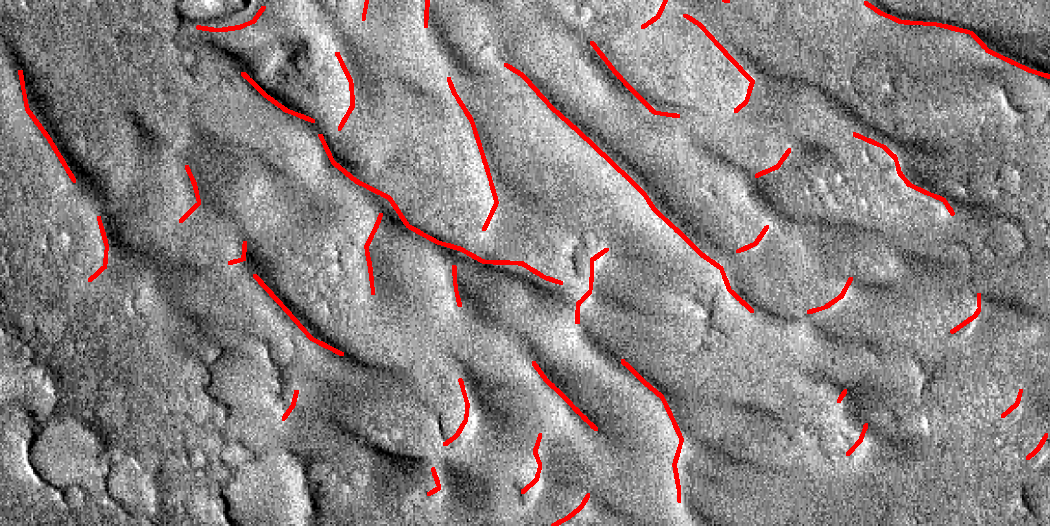
\includegraphics[width=\textwidth]{figures/area13_with_gt}
		\caption{  Region 13 }
		\label{fig:area13_image}
	\end{subfigure}
	\begin{subfigure}[b]{0.3\textwidth}
		\centering
		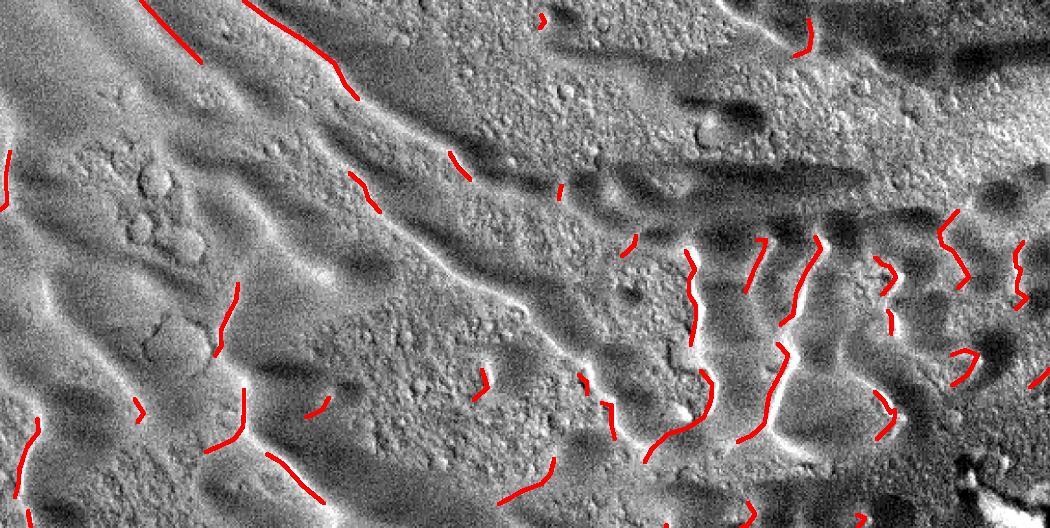
\includegraphics[width=\textwidth]{figures/area15_with_gt}
		\caption{  Region 15 }
		\label{fig:area15_image}
	\end{subfigure}

	\caption{Ganges Chasms Mars dataset from \cite{vaz_object_based_dune_analysis} which includes 14 regions extracted with the ground truth labeled. }
	\label{fig:mars_ganges_dataset}
\end{figure*}



The dataset is essentially a CTX mosaic of the Ganges chasma, which spans an area of 500 km\textsuperscript{2}, and includes a wide variety of dune types and morphologies. According to \cite{fenton_aeolian_sediment_ganges_chasma_mars}, many aeolian fatures can be found in the Ganges Chasma. Sand sheets, dune fields, unidirectional features such as barchan dunes were all identified within this region. The overall structure of the Ganges dune field is a complex set of many diverging dunes, which makes it a challenging and appropriate area for testing this method. 


\subsection{Evaluation}\label{subsec:evaluation}

For each method, a number of metrics were used to evaluate the quality of each dune detector. A true positive (\emph{TP}) is defined as a positively detected crest-lines. A detection is determined to be positive if it contains a ground truth within a radius of $\epsilon$. A false positive (\emph{FP}) is defined to be a detection which is not an actual dune crest-line. A false positive occurs when a detection does not have a ground truth crest-line within a radius of $\epsilon$. A false negative (\emph{FN}) is an actual ground truth crest-line which was no identified. A false negative occurs when no detection is found within a radius of $\epsilon$.

Determining an appropriate value for $\epsilon$ affects the overall results as well. Based on the datasets used in this research, and accounting for error in labeling and image resolution, an appropriate value was chosen to be $\epsilon=10$ (pixels). If the scale of the image is known (meters per pixel), pixels can be converted to a more meaningful metric scale.

\emph{Precision} is the ratio of correct detection to overall detection. It measures how precise the detections are. It can be computed from the true positives and false positives by $P=TP/(TP+FP)$. \emph{Recall} Recall is the percentage of crest-lines identified. It can be computed from the true positives and false negatives using $R=TP/(TP+FN)$. \emph{Angular Error} The difference between the dune field average orientation computed from the detected crest-lines, and the average orientation computed from the ground truth crest-lines (in degrees), represented by $\Delta_{\theta}$. Finally, the \emph{Inter-Dune Distance Error} The difference between the dune distance computed from the detected crest-lines and the distance computed from the ground truth crest-lines (in pixels), represented by $\Delta_{d}$.

Additionally, the terrestrial dataset includes many representative regions with various dune types. There are two options for training models:
\begin{description}
	\item[Unique Model Per Region] In this approach, a machine learning model is trained for each region. The result are more accurate within each regions, but the solution is not as generalized. 
	\item[Cross-Region Model] In this approach, a single model is trained using all regions. The results produced are typically less accurate than the unique model per region approach, but provides a more generalized solution.
\end{description}

Another dataset evaluated was the Mars dataset from section \ref{subsec:mars_dataset}. Included are the results from the research done in \cite{vaz_object_based_dune_analysis}, which includes the ground truth and results. Our machine learning method was compared side-by-side with the results from \cite{vaz_object_based_dune_analysis} on each of the 16 regions sampled. The 16 regions are split half and half for training and testing respectively, where odd regions were used for training and even regions for testing. 

\subsection{Results} \label{subsec:results-and-discussion}
The machine learning approaches require the training of the models using a set of data and the model is then tested on a separate set of data. Therefore, a separate set of data was created to evaluate the performance of the machine learning approach, shown in Figure \ref{fig:terrestrial_test_dataset}.


The addition of the test images allows us to better evaluate the effectiveness of the various models and methods used to train the machine learning system. To train each model a set of data is collected from the both the training and test sets using the method described in section \ref{subsubsec:dataset_creation}. A set of pixels are randomly selected for each image, preserving a equal count of crest-line pixels and non-crest-line pixels. Crest-line pixels are determined using the provided ground truth. The number of pixels extracted was varied to determine the effectiveness of the model. When fewer data was used, the model could be trained very quickly but the representation of the model achieved poorer results. A larger training set provided a much better representation of crest-lines, at the cost of efficiency. The number of pixels used found to be optimal was in the range of 1000 to 5000.

As described in section \ref{subsubsec:feature_descriptor_extraction}, the features were extracted at each sampled pixel. Many feature types were used including BRIEF, ORB, BRISK, SURF, HOG, LBPH, and even using raw pixel values but the SIFT performance was far superior to all others. The traditional 128 bin SIFT descriptor vector was extracted at each pixel as the feature to use for the model.

The next consideration is the type of machine learning classifier to use for the model. Again, as described in section \ref{subsubsec:supervised_learning_classifiers}, there are many classifier options available such as Bayesian, Neural Networks, Decision Trees, Support Vector Machines.

\begin{table*}
	\centering
	\caption{True positive and false positive rates results of the training process to build the crest-line GBT classifier model using the SIFT descriptors, for building response maps }
%	\label{tab:classifier_training_test_results}
%	\begin{subtable}{0.98\textwidth}
%		\centering
%		\begin{tabu} to 0.9\textwidth { | X[2,c] || X[1,c] | X[1,c] || X[1,c] | X[1,c] | }
%			\hline
%			\multirow{2}{*}{\textbf{SVM Results}} & \multicolumn{2}{c||}{\textbf{Training Set}} &  \multicolumn{2}{c|}{\textbf{Test Set}} \\
%			\cline{2-5}
%			& \textbf{TPR} & \textbf{FPR} & \textbf{TPR} & \textbf{FPR} \\
%			\hline
%			Kalahari & 0.9939 & 0.0151 & 0.8703 & 0.1383 \\
%			Namib & 0.9896 & 0.0183 & 0.9054 & 0.1300 \\
%			Simpson & 0.9959 & 0.0078 & 0.7950 & 0.1584 \\
%			Skeleton Coast & 0.9917 & 0.0195 & 0.8031 & 0.1393 \\
%			WDC & 1.0000 & 0.0018 & 0.6421 & 0.1874 \\
%			White Sands & 0.9913 & 0.0099 & 0.7081 & 0.1495 \\
%			\hline
%		\end{tabu}
%		\caption{Support Vector Machine Results}
%		\label{tab:svm_training_test_results}
%	\end{subtable}
%	\begin{subtable}{0.98\textwidth}
%		\centering
%		\begin{tabu} to 0.9\textwidth { | X[2,c] || X[1,c] | X[1,c] || X[1,c] | X[1,c] | }
%			\hline
%			\multirow{2}{*}{\textbf{Normal Bayes Results}} & \multicolumn{2}{c||}{\textbf{Training Set}} &  \multicolumn{2}{c|}{\textbf{Test Set}} \\
%			\cline{2-5}
%			& \textbf{TPR} & \textbf{FPR} & \textbf{TPR} & \textbf{FPR} \\
%			\hline
%			Kalahari & 1.0000 & 0.0491 & 0.4440 & 0.0468 \\
%			Namib & 0.9913 & 0.0754 & 0.6359 & 0.1081 \\
%			Simpson & 0.9937 & 0.0428 & 0.6015 & 0.0823 \\
%			Skeleton Coast & 0.9959 & 0.1074 & 0.5714 & 0.1045 \\
%			WDC & 0.9950 & 0.0499 & 0.8511 & 0.1624 \\
%			White Sands & 0.9978 & 0.0812 & 0.5483 & 0.1111 \\
%			\hline
%		\end{tabu}
%		\caption{Normal Bayes Classifier Results}
%		\label{tab:bayes_training_test_results}
%	\end{subtable}
%	\begin{subtable}{0.98\textwidth}
%		\centering
%		\begin{tabu} to 0.9\textwidth { | X[2,c] || X[1,c] | X[1,c] || X[1,c] | X[1,c] | }
%			\hline
%			\multirow{2}{*}{\textbf{Random Tree Results}} & \multicolumn{2}{c||}{\textbf{Training Set}} &  \multicolumn{2}{c|}{\textbf{Test Set}} \\
%			\cline{2-5}
%			& \textbf{TPR} & \textbf{FPR} & \textbf{TPR} & \textbf{FPR} \\
%			\hline
%			Kalahari & 0.9837 & 0.0981 & 0.9037 & 0.1277 \\
%			Namib & 0.9809 & 0.1181 & 0.9504 & 0.1493 \\
%			Simpson & 0.9586 & 0.0895 & 0.8317 & 0.2078 \\
%			Skeleton Coast & 0.9793 & 0.1191 & 0.8764 & 0.1844 \\
%			WDC & 0.8856 & 0.0942 & 0.7107 & 0.2048 \\
%			White Sands & 0.9524 & 0.0990 & 0.7955 & 0.1960 \\
%			\hline
%		\end{tabu}
%		\caption{Random Trees Classifier Results}
%		\label{tab:random_trees_training_test_results}
%	\end{subtable}
	\begin{subtable}{0.98\textwidth}
		\centering
		\begin{tabu} to 0.9\textwidth { | X[2,c] || X[1,c] | X[1,c] || X[1,c] | X[1,c] | }
			\hline
			\multirow{2}{*}{\textbf{GBT Model Results}} & \multicolumn{2}{c||}{\textbf{Training Set}} &  \multicolumn{2}{c|}{\textbf{Test Set}} \\
			\cline{2-5}
			& \textbf{TPR} & \textbf{FPR} & \textbf{TPR} & \textbf{FPR} \\
			\hline
			Kalahari & 0.9817 & 0.0792 & 0.8900 & 0.1213 \\
			Namib & 0.9688 & 0.1201 & 0.9267 & 0.1415 \\
			Simpson & 0.9400 & 0.0972 & 0.8279 & 0.1975 \\
			Skeleton Coast & 0.9813 & 0.1133 & 0.8764 & 0.1762 \\
			WDC & 0.8706 & 0.0943 & 0.7090 & 0.1895 \\
			White Sands & 0.9351 & 0.1129 & 0.7677 & 0.1636 \\
			\hline
		\end{tabu}
		\caption{Gradient Boosted Trees Results}
		\label{tab:boosted_trees_training_test_results}
	\end{subtable}
\end{table*}

In Table \ref{tab:classifier_training_test_results} shows the results of the training process. The results show that SVM and the decision trees perform the best. The Normal Bayes classifier has a tendency to over-fit the training data. This is evident by the fact that it learns the training data very well but has poor performance on the test set. Overall, the Gradient Boosted Tree results shown in Table \ref{tab:boosted_trees_training_test_results} has the best results.

Next, the machine learning method results (using Gradient Boosted Trees on the extracted SIFT descriptors) explained in section \ref{subsec:machine_learning_approach} are discussed. The method was applied in two experiments: 

\begin{enumerate}
	\item Training one model for each region: For each region, training data and test data was collected, and a single model is created and trained for that specific region. The results of this approach are shown in Table \ref{tab:machine_learning_approach_results}.
	\item Cross-Region model: A single model is used for all the regions. The training data was collected from all regions, the model was trained using the features from all the regions. The results of this approach are shown in Table \ref{tab:cross_region_machine_learning_approach_results}
\end{enumerate}

\begin{table}
	\centering
	\caption{Results of the machine learning method presented in section \ref{subsec:machine_learning_approach} using a single Gradient Boosted Tree classifier and the SIFT features trained across all the regions, inludes the Precision and Recall (a) and the Dune Metrics error results (b) for both the training and test image sets. }
	\label{tab:cross_region_machine_learning_approach_results}
	\begin{subtable}{0.98\textwidth}
		\centering
		\begin{tabu} to 0.9\textwidth { | X[2,c] || X[1,c] | X[1,c] || X[1,c] | X[1,c] | }
			\hline
			\multirow{2}{*}{\textbf{Datasets}} & \multicolumn{2}{c||}{\textbf{Training Set}} &  \multicolumn{2}{c|}{\textbf{Test Set}} \\
			\cline{2-5}
			& \textbf{Precision} & \textbf{Recall} & \textbf{Precision} & \textbf{Recall} \\
			\hline
			Kalahari & 0.9379 & 0.9726 & 0.7694 & 0.9232 \\
			Namib & 0.8491 & 0.9676 & 0.7867 & 0.8778 \\
			Simpson & 0.9084 & 0.9249 & 0.7658 & 0.8398 \\
			Skeleton Coast & 0.7632 & 0.9536 & 0.7938 & 0.9393 \\
			WDC & 0.8981 & 0.8554 & 0.7558 & 0.8559 \\
			White Sands & 0.9370 & 0.8784 & 0.8695 & 0.8001 \\
			\hline
		\end{tabu}
		\caption{Machine Learning Precision and Recall Results (GBT-SIFT)}
		\label{tab:machine_learning_PR}
	\end{subtable}
	\begin{subtable}{0.98\textwidth}
		\centering
		\begin{tabu} to 0.9\textwidth { | X[2,c] || X[1,c] | X[1,c] || X[1,c] | X[1,c] | }
			\hline
			\multirow{2}{*}{\textbf{Datasets}} & \multicolumn{2}{c||}{\textbf{Training Set}} &  \multicolumn{2}{c|}{\textbf{Test Set}} \\
			\cline{2-5}
			& \textbf{$\Delta_{\theta}$} & \textbf{$\Delta_{d}$ (Pixels)} & \textbf{$\Delta_{\theta}$} & \textbf{$\Delta_{d}$ (Pixels)} \\
			\hline
			Kalahari & 0.2437\textdegree & 3.9228 & 1.5047\textdegree & 7.6993 \\
			Namib & 8.0655\textdegree & 13.2756 & 2.8757\textdegree & 4.0135 \\
			Simpson & 13.0593\textdegree & 8.3083 & 0.7329\textdegree & 2.4516 \\
			Skeleton Coast & 0.0434\textdegree & 9.5747 & 1.4801\textdegree & 1.5155 \\
			WDC & 1.9937\textdegree & 1.9692 & 2.1001\textdegree & 1.7801 \\
			White Sands & 10.6052\textdegree & 4.3457 & 2.5835\textdegree & 7.8096 \\
			\hline
		\end{tabu}
		\caption{Dune Metrics Results for Angular Error ($\Delta_{\theta}$) and Inter-Dune Distance Error ($\Delta_{d}$) }
		\label{tab:machine_learning_metrics_error}
	\end{subtable}
	\caption{Results of the machine learning method presented in section \ref{subsec:machine_learning_approach} using the Gradient Boosted Tree classifier and the SIFT features, includes the Precision and Recall (a) and the Dune Metrics error results (b) for both the training and test image sets. }
	\label{tab:machine_learning_approach_results}
\end{table}

\begin{table}
	\centering
	\begin{subtable}{0.98\textwidth}
		\centering
		\begin{tabu} to 0.9\textwidth { | X[2,c] || X[1,c] | X[1,c] || X[1,c] | X[1,c] | }
			\hline
			\multirow{2}{*}{\textbf{Datasets}} & \multicolumn{2}{c||}{\textbf{Training Set}} &  \multicolumn{2}{c|}{\textbf{Test Set}} \\
			\cline{2-5}
			& \textbf{Precision} & \textbf{Recall} & \textbf{Precision} & \textbf{Recall} \\
			\hline
			Kalahari & 0.9258 & 0.9254 & 0.7300 & 0.8444 \\
			Namib & 0.7942 & 0.9590 & 0.6637 & 0.8634 \\
			Simpson & 0.8491 & 0.7854 & 0.7375 & 0.7579 \\
			Skeleton Coast & 0.5768 & 0.9096 & 0.6135 & 0.8967 \\
			WDC & 0.9315 & 0.6155 & 0.8585 & 0.5771 \\
			White Sands & 0.9374 & 0.6431 & 0.7909 & 0.3973 \\
			\hline
		\end{tabu}
		\caption{Machine Learning Precision and Recall Cross-Region Results (GBT-SIFT)}
		\label{tab:cross_region_machine_learning_PR}
	\end{subtable}
	\begin{subtable}{0.98\textwidth}
		\centering
		\begin{tabu} to 0.9\textwidth { | X[2,c] || X[1,c] | X[1,c] || X[1,c] | X[1,c] | }
			\hline
			\multirow{2}{*}{\textbf{Datasets}} & \multicolumn{2}{c||}{\textbf{Training Set}} &  \multicolumn{2}{c|}{\textbf{Test Set}} \\
			\cline{2-5}
			& \textbf{$\Delta_{\theta}$} & \textbf{$\Delta_{d}$ (Pixels)} & \textbf{$\Delta_{\theta}$} & \textbf{$\Delta_{d}$ (Pixels)} \\
			\hline
			Kalahari & 0.4803\textdegree & 5.0142 & 1.0343\textdegree & 5.9187 \\
			Namib & 2.8976\textdegree & 16.7863 & 9.5319\textdegree & 2.4645 \\
			Simpson & 13.938\textdegree & 9.0225 & 0.2434\textdegree & 2.7176 \\
			Skeleton Coast & 10.4224\textdegree & 18.6251 & 7.7421\textdegree & 8.3473 \\
			WDC & 12.7138\textdegree & 11.1957 & 15.8434\textdegree & 21.4145 \\
			White Sands & 11.0979\textdegree & 15.9853 & 1.2744\textdegree & 53.3311 \\
			\hline
		\end{tabu}
		\caption{Dune Metrics Results for Angular Error ($\Delta_{\theta}$) and Inter-Dune Distance Error ($\Delta_{d}$) for Cross-Region}
		\label{tab:cross_region_machine_learning_metrics_error}
	\end{subtable}
\end{table}

The results clearly show that the cross-region model struggles at learning the general concept of a dune across many regions. The precision and recall values of the single model per region approach shown in Table \ref{tab:machine_learning_PR} are measurably better than the cross-region approach results shown in Table \ref{tab:cross_region_machine_learning_PR}. The difference is especially large with complex dune structures such as the Winnemucca Dune Complex and the White Sands regions. The dune metrics computed in Tables \ref{tab:machine_learning_metrics_error} and \ref{tab:cross_region_machine_learning_metrics_error} are also much worse, since the calculation of these metrics heavily depends on accurate detection of crest-lines.  

\begin{figure}
	\centering
	\begin{subfigure}{0.48\textwidth}
		\centering
		%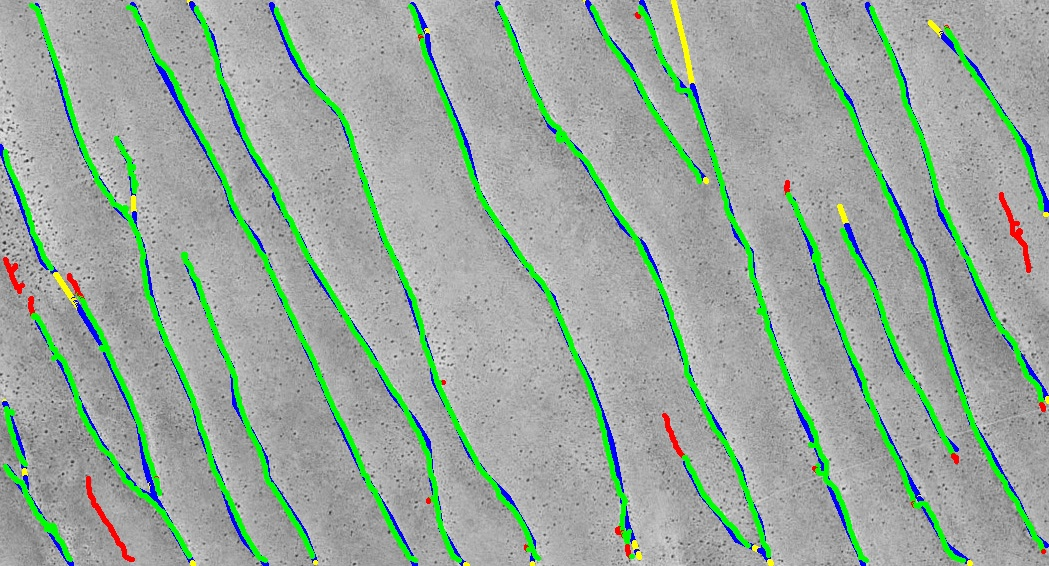
\includegraphics[width=1.0\linewidth]{figures/ml_kalahari_results}
		\caption{ Kalahari Training }
		\label{fig:ml_kalahari_results}
	\end{subfigure}
	\begin{subfigure}{0.48\textwidth}
		\centering
		%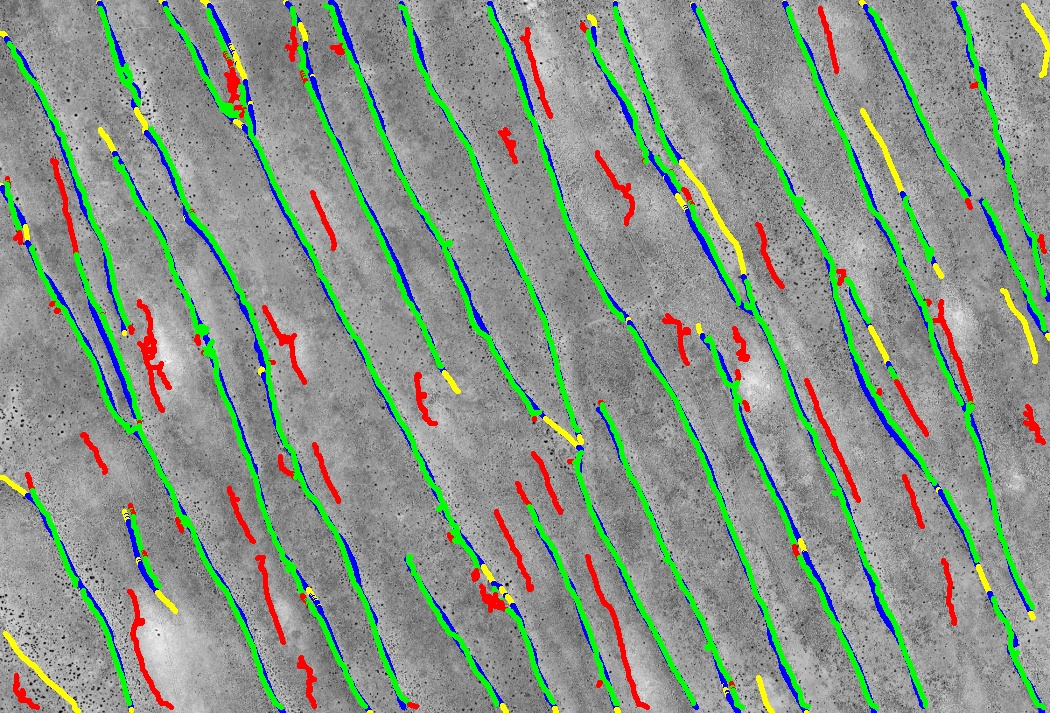
\includegraphics[width=1.0\linewidth]{figures/ml_kalahari_test_results}
		\caption{ Kalahari Test }
		\label{fig:ml_kalahari_test_results}
	\end{subfigure}
	\begin{subfigure}{0.48\textwidth}
		\centering
		%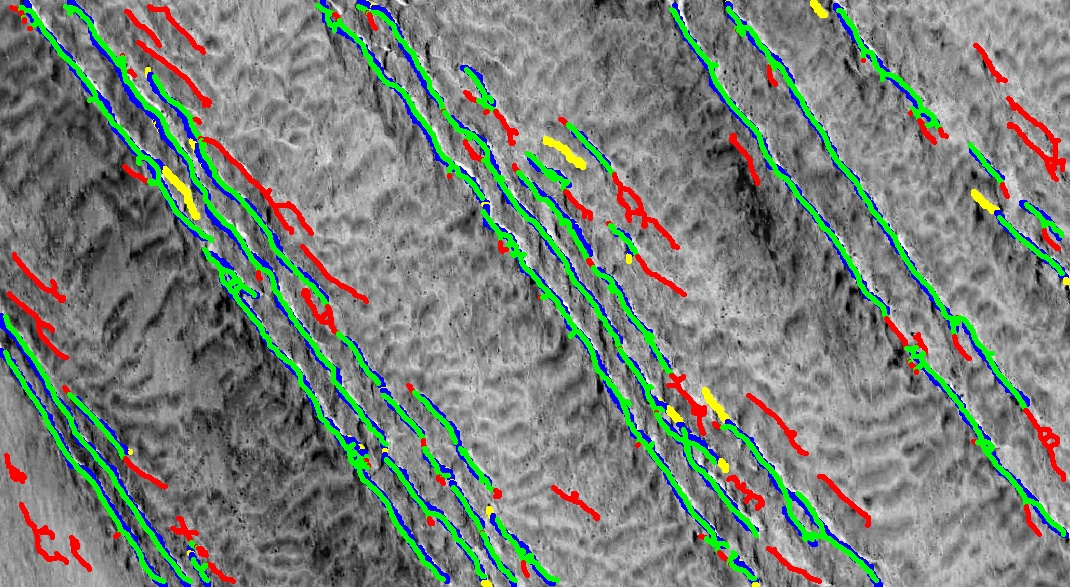
\includegraphics[width=1.0\linewidth]{figures/ml_namib_results}
		\caption{ Namib Training }
		\label{fig:ml_namib_results}
	\end{subfigure}
	\begin{subfigure}{0.48\textwidth}
		\centering
		%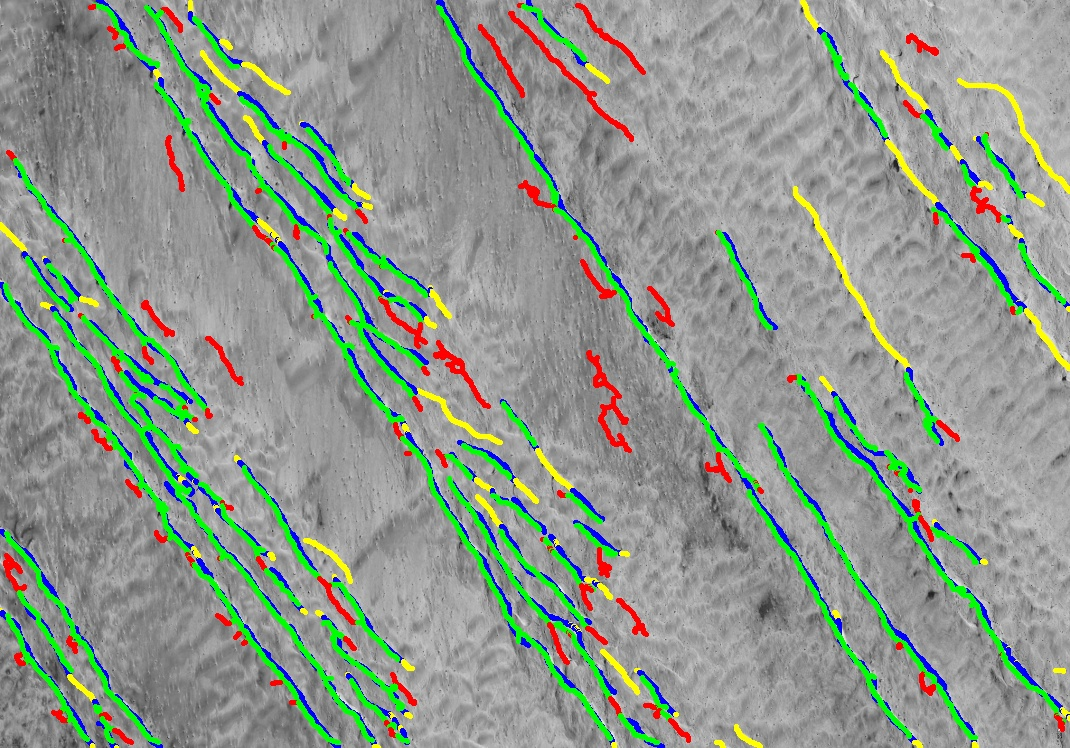
\includegraphics[width=1.0\linewidth]{figures/ml_namib_test_results}
		\caption{ Namib Test }
		\label{fig:ml_namib_test_results}
	\end{subfigure}
	\begin{subfigure}{0.48\textwidth}
		\centering
		%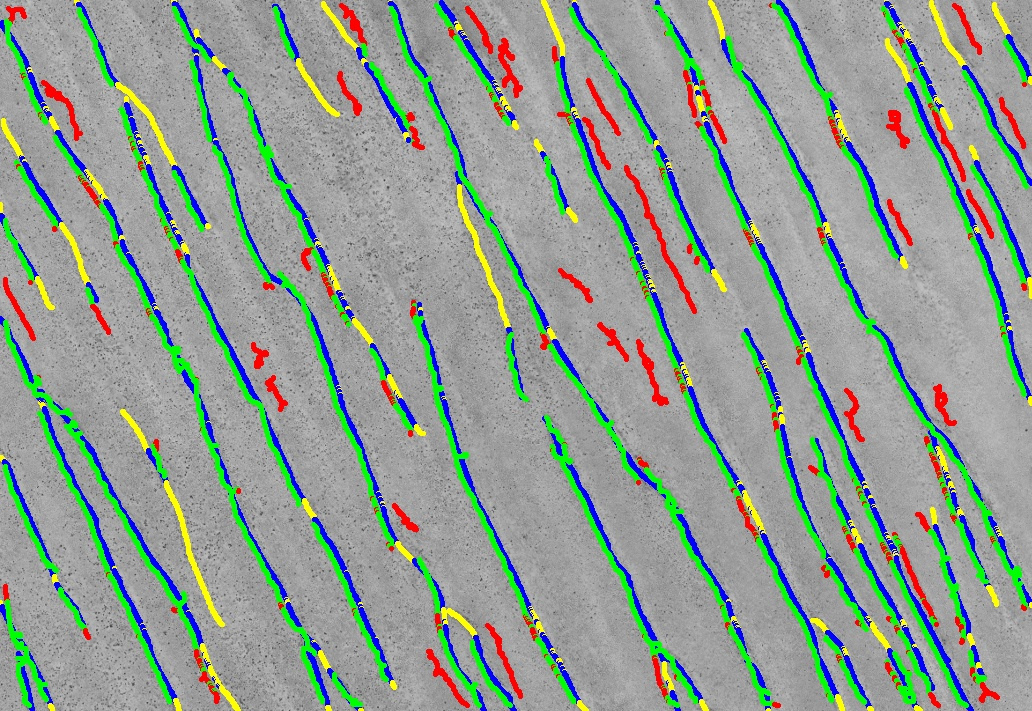
\includegraphics[width=1.0\linewidth]{figures/ml_simpson_results}
		\caption{ Simpson Training }
		\label{fig:ml_simpson_results}
	\end{subfigure}
	\begin{subfigure}{0.48\textwidth}
		\centering
		%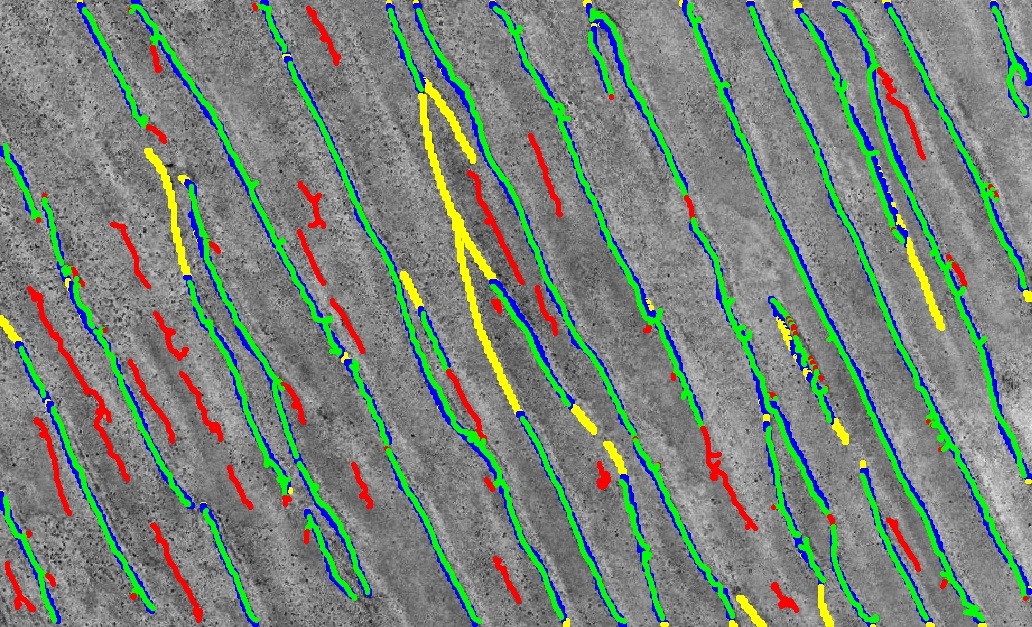
\includegraphics[width=1.0\linewidth]{figures/ml_simpson_test_results}
		\caption{ Simpson Test }
		\label{fig:ml_simpson_test_results}
	\end{subfigure}
\end{figure}
\begin{figure}
	\ContinuedFloat
	\centering
	\begin{subfigure}{0.48\textwidth}
		\centering
		%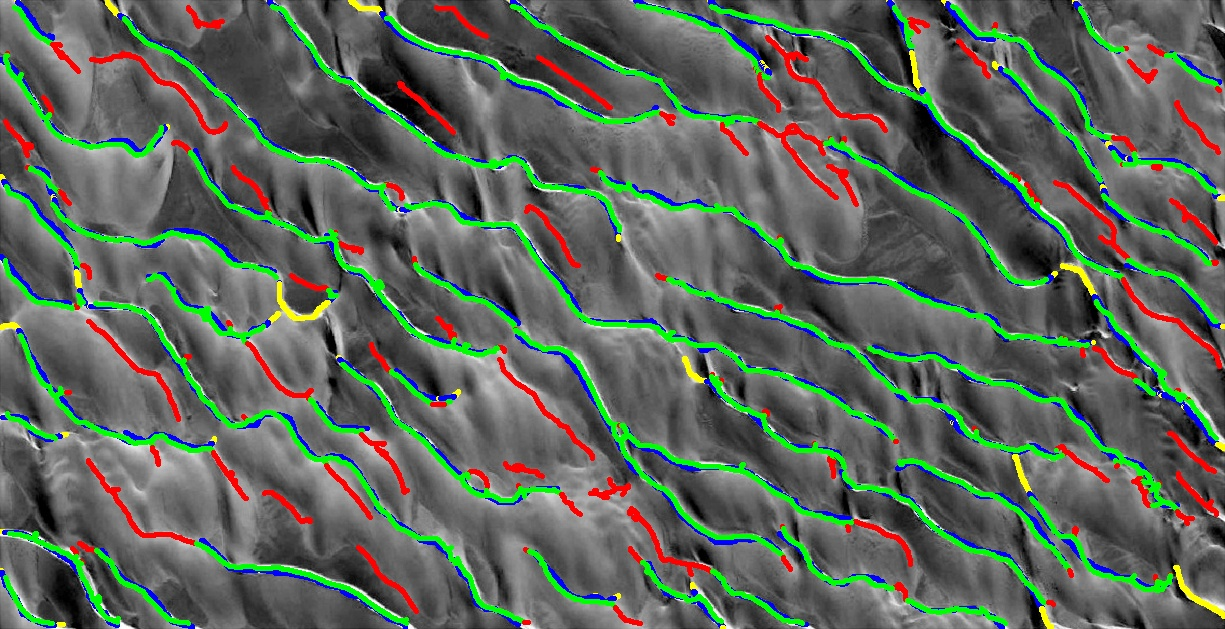
\includegraphics[width=1.0\linewidth]{figures/ml_skeleton_coast_results}
		\caption{ Skeleton Coast Training }
		\label{fig:ml_skeleton_coast_results}
	\end{subfigure}
	\begin{subfigure}{0.48\textwidth}
		\centering
		%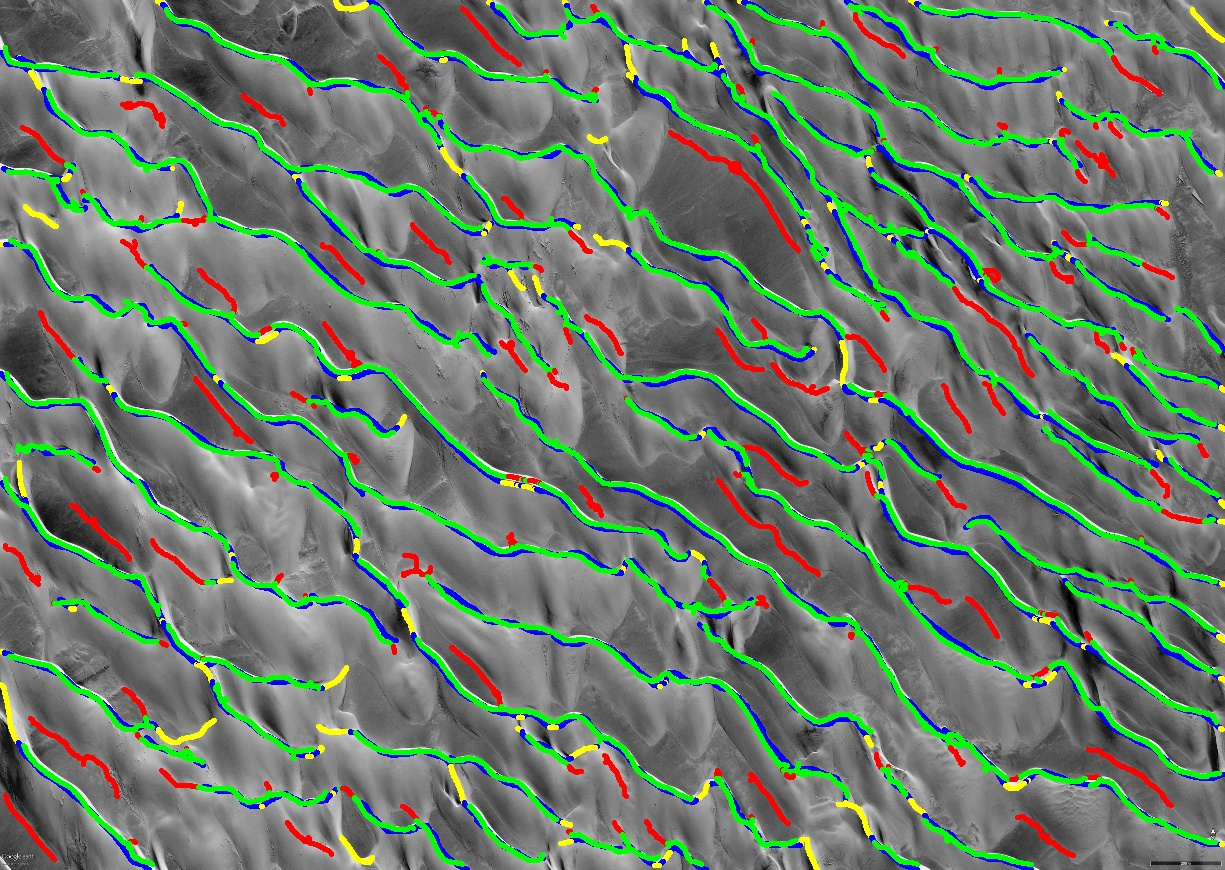
\includegraphics[width=1.0\linewidth]{figures/ml_skeleton_coast_test_results}
		\caption{ Skeleton Coast Test }
		\label{fig:ml_skeleton_coast_test_results}
	\end{subfigure}
	\begin{subfigure}{0.48\textwidth}
		\centering
		%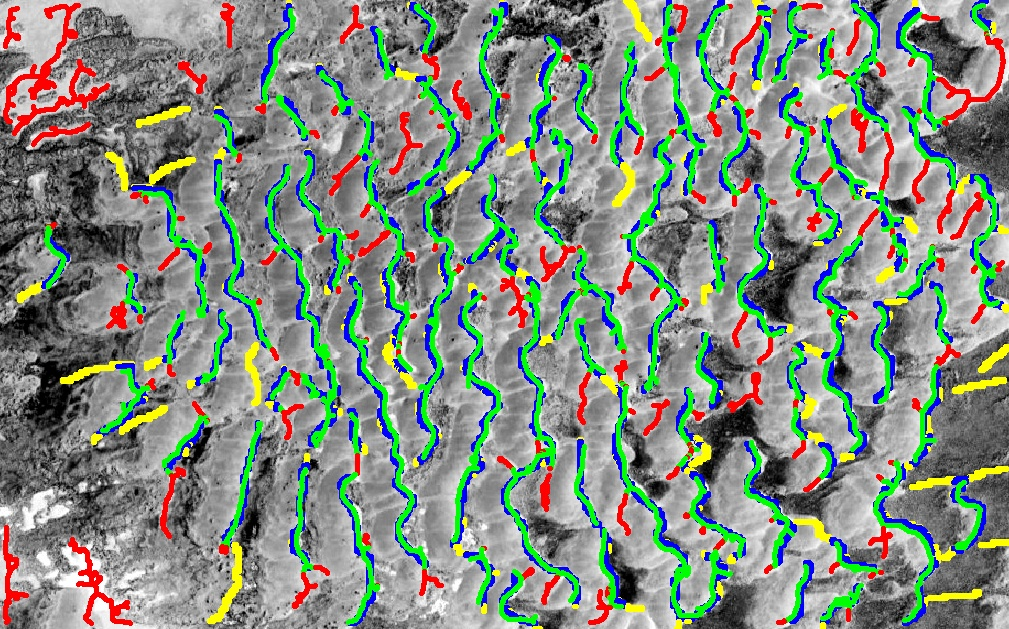
\includegraphics[width=1.0\linewidth]{figures/ml_wdc_results}
		\caption{ WDC Training }
		\label{fig:ml_wdc_results}
	\end{subfigure}
	\begin{subfigure}{0.48\textwidth}
		\centering
		%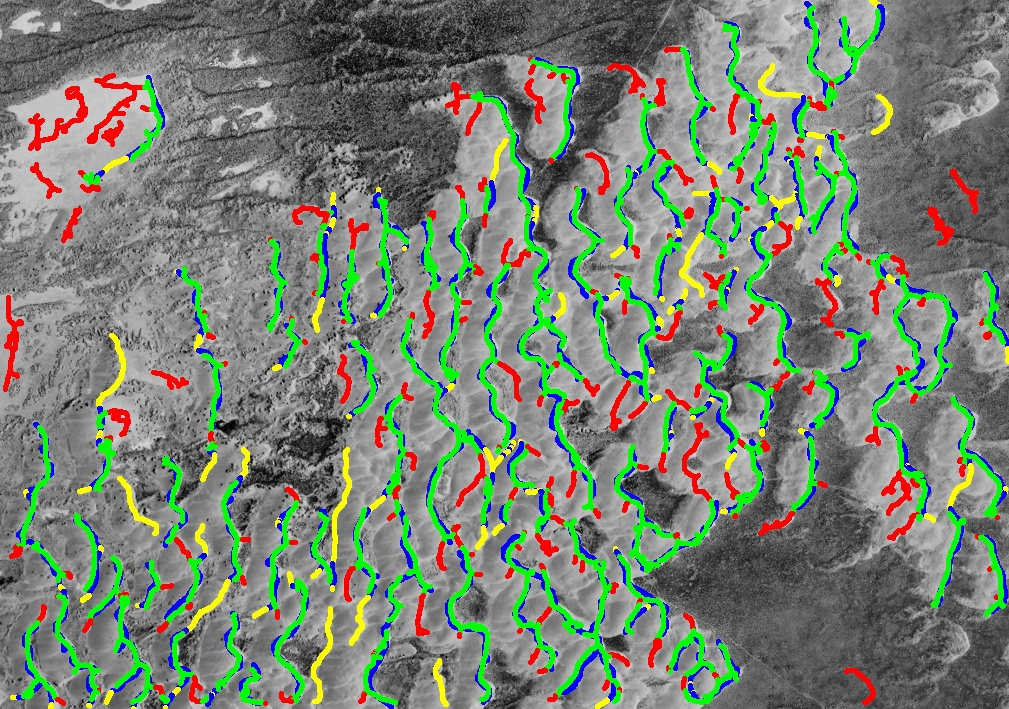
\includegraphics[width=1.0\linewidth]{figures/ml_wdc_test_results}
		\caption{ WDC Test }
		\label{fig:ml_wdc_test_results}
	\end{subfigure}
	\begin{subfigure}{0.48\textwidth}
		\centering
		%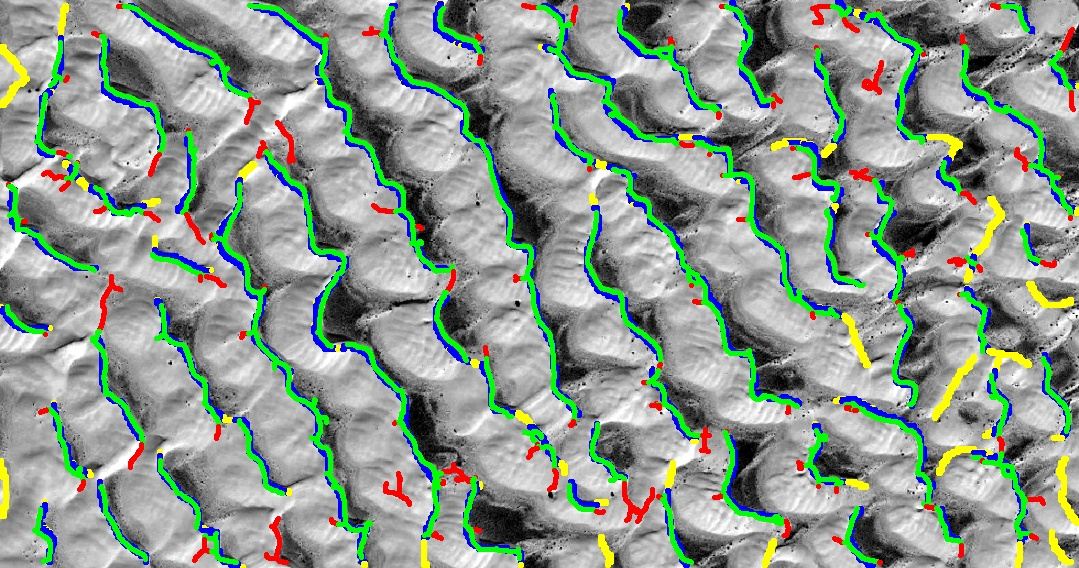
\includegraphics[width=1.0\linewidth]{figures/ml_white_sands_results}
		\caption{ White Sands Training }
		\label{fig:ml_white_sands_results}
	\end{subfigure}
	\begin{subfigure}{0.48\textwidth}
		\centering
		%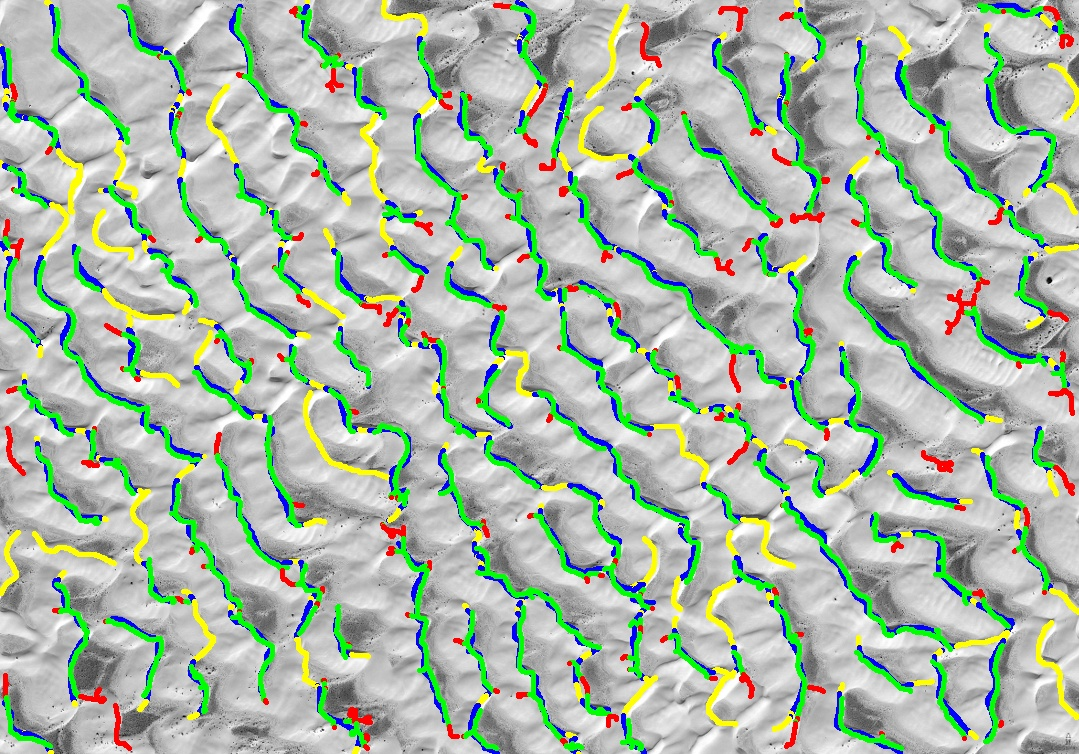
\includegraphics[width=1.0\linewidth]{figures/ml_white_sands_test_results}
		\caption{ White Sands Test }
		\label{fig:ml_white_sands_test_results}
	\end{subfigure}
	\caption{ The results of the  crest-line detection for the machine learning approach on terrestrial dataset for both the training images \subref{fig:ml_kalahari_results}, \subref{fig:ml_namib_results}, \subref{fig:ml_simpson_results}, \subref{fig:ml_skeleton_coast_results}, \subref{fig:ml_wdc_results}, \subref{fig:ml_white_sands_results}, and the test images \subref{fig:ml_kalahari_test_results}, \subref{fig:ml_namib_test_results}, \subref{fig:ml_simpson_test_results}, \subref{fig:ml_skeleton_coast_test_results}, \subref{fig:ml_wdc_test_results}, \subref{fig:ml_white_sands_test_results} using the GBT classifier and SIFT features. \underline{\textbf{Legend}}: \emph{Green} - True Positives, \emph{Red} - False Positives, \emph{Yellow} - False Negatives, \emph{Blue} - Ground truth correctly detected.  }
	\label{fig:ml_results}
\end{figure}

The results of the machine learning crest-line detection are shown in Figure \ref{fig:ml_results}. The true positive detections are shown in green, along with the correctly identified ground truth in blue. The false negatives (crest-lines not correctly detected) are shown in yellow, and false positives are shown in red. The results show that the overall performance of this approach is quite good. 

One important point to note is that there are inaccuracies in the ground truth itself. In many cases, some false positives may not actually be false positives because some crest-lines where not labeled in the ground truth. Additionally, some false negatives may be caused by poor localization of the ground truth labels. For the most part, the ground truth is fairly accurate, but a second pass at labeling would increase the overall precision and recall rates results.

\subsubsection*{Mixed Machine Learning and Gradient Orientation Approach Results}

The final results presented are for the mixed machine learning and gradient orientation approach presented in section \ref{subsec:mixed_ml_gradient_approach}. The approach essentially combines the methods from sections \ref{subsec:gradient_orientation_based} and \ref{subsec:machine_learning_approach} to yield improved results. Similarly to the previous method, the machine learning model in this approach can also be trained for each region or across all the regions. The results of these methods are presented in Tables \ref{tab:ml_grad_approach_results} and \ref{tab:cross_region_ml_grad_approach_results}. The results projected onto the images are shown in Figure \ref{fig:mixed_ml_grad_results}.

\begin{table}
	\centering
	\caption{Results of the mixed machine learning and gradient-based method presented in section \ref{subsec:mixed_ml_gradient_approach} using the Gradient Boosted Tree classifier and the SIFT features, includes the Precision and Recall (a) and the Dune Metrics error results (b) for both the training and test image sets. }
	\label{tab:ml_grad_approach_results}
	\begin{subtable}{0.98\textwidth}
		\centering
		\begin{tabu} to 0.9\textwidth { | X[2,c] || X[1,c] | X[1,c] || X[1,c] | X[1,c] | }
			\hline
			\multirow{2}{*}{\textbf{Datasets}} & \multicolumn{2}{c||}{\textbf{Training Set}} &  \multicolumn{2}{c|}{\textbf{Test Set}} \\
			\cline{2-5}
			& \textbf{Precision} & \textbf{Recall} & \textbf{Precision} & \textbf{Recall} \\
			\hline
			Kalahari & 0.9523 & 0.9904 & 0.9003 & 0.8979 \\
			Namib & 0.9512 & 0.9831 & 0.9366 & 0.8443 \\
			Simpson & 0.9542 & 0.8341 & 0.9111 & 0.8335 \\
			Skeleton Coast & 0.9356 & 0.9806 & 0.9829 & 0.8974 \\
			WDC & 0.9711 & 0.7996 & 0.9145 & 0.8006 \\
			White Sands & 0.9789 & 0.8328 & 0.9540 & 0.7948 \\
			\hline
		\end{tabu}
		\caption{Mixed ML/Grad Precision and Recall Results (GBT-SIFT)}
		\label{tab:ml_grad_PR}
	\end{subtable}
	\begin{subtable}{0.98\textwidth}
		\centering
		\begin{tabu} to 0.9\textwidth { | X[2,c] || X[1,c] | X[1,c] || X[1,c] | X[1,c] | }
			\hline
			\multirow{2}{*}{\textbf{Datasets}} & \multicolumn{2}{c||}{\textbf{Training Set}} &  \multicolumn{2}{c|}{\textbf{Test Set}} \\
			\cline{2-5}
			& \textbf{$\Delta_{\theta}$} & \textbf{$\Delta_{d}$ (Pixels)} & \textbf{$\Delta_{\theta}$} & \textbf{$\Delta_{d}$ (Pixels)} \\
			\hline
			Kalahari & 0.5643\textdegree & 8.4518 & 0.5811\textdegree & 9.4325 \\
			Namib & 6.2212\textdegree & 2.36 & 3.5316\textdegree & 19.8735 \\
			Simpson & 12.5965\textdegree & 9.8947 & 1.0102\textdegree & 5.3046 \\
			Skeleton Coast & 0.5231\textdegree & 5.2738 & 1.9851\textdegree & 16.7215 \\
			WDC & 2.6216\textdegree & 6.4317 & 4.0554\textdegree & 6.8127 \\
			White Sands & 10.2219\textdegree & 10.2207 & 17.0219\textdegree & 14.2709 \\
			\hline
		\end{tabu}
		\caption{Dune Metrics Results for Angular Error ($\Delta_{\theta}$) and Inter-Dune Distance Error ($\Delta_{d}$) }
		\label{tab:ml_grad_metrics_error}
	\end{subtable}
\end{table}

\begin{table}
	\centering
	\caption{Results of the mixed machine learning and gradient-based method presented in section \ref{subsec:mixed_ml_gradient_approach} using the Gradient Boosted Tree classifier and the SIFT features trained across all the regions, includes the Precision and Recall \subref{tab:cross_region_ml_grad_PR} and the Dune Metrics error results \subref{tab:cross_region_ml_grad_metrics_error} for both the training and test image sets. }
	\label{tab:cross_region_ml_grad_approach_results}
	\begin{subtable}{0.98\textwidth}
		\centering
		\begin{tabu} to 0.9\textwidth { | X[2,c] || X[1,c] | X[1,c] || X[1,c] | X[1,c] | }
			\hline
			\multirow{2}{*}{\textbf{Datasets}} & \multicolumn{2}{c||}{\textbf{Training Set}} &  \multicolumn{2}{c|}{\textbf{Test Set}} \\
			\cline{2-5}
			& \textbf{Precision} & \textbf{Recall} & \textbf{Precision} & \textbf{Recall} \\
			\hline
			Kalahari & 0.9502 & 0.9908 & 0.9007 & 0.9244 \\
			Namib & 0.9336 & 0.9705 & 0.8926 & 0.9137 \\
			Simpson & 0.8833 & 0.8117 & 0.7108 & 0.7943 \\
			Skeleton Coast & 0.8946 & 0.9089 & 0.9284 & 0.8740 \\
			WDC & 0.9906 & 0.4903 & 0.9780 & 0.3942 \\
			White Sands & 1.000 & 0.3122 & 0.9930 & 0.1347 \\
			\hline
		\end{tabu}
		\caption{Mixed ML/Grad Precision and Recall Results (GBT-SIFT)}
		\label{tab:cross_region_ml_grad_PR}
	\end{subtable}
	\begin{subtable}{0.98\textwidth}
		\centering
		\begin{tabu} to 0.9\textwidth { | X[2,c] || X[1,c] | X[1,c] || X[1,c] | X[1,c] | }
			\hline
			\multirow{2}{*}{\textbf{Datasets}} & \multicolumn{2}{c||}{\textbf{Training Set}} &  \multicolumn{2}{c|}{\textbf{Test Set}} \\
			\cline{2-5}
			& \textbf{$\Delta_{\theta}$} & \textbf{$\Delta_{d}$ (Pixels)} & \textbf{$\Delta_{\theta}$} & \textbf{$\Delta_{d}$ (Pixels)} \\
			\hline
			Kalahari & 0.5742\textdegree & 0.1654 & 0.1318\textdegree & 2.1444 \\
			Namib & 4.9791\textdegree & 0.9722 & 5.7731\textdegree & 11.1356 \\
			Simpson & 14.0118\textdegree & 15.2678 & 0.4280\textdegree & 14.03 \\
			Skeleton Coast & 2.8091\textdegree & 2.6331 & 1.3421\textdegree & 11.9770 \\
			WDC & 7.3042\textdegree & 45.1448 & 6.8027\textdegree & 63.6407 \\
			White Sands & 11.8688\textdegree & 74.6094 & 12.6240\textdegree & 112.5056 \\
			\hline
		\end{tabu}
		\caption{Dune Metrics Results for Angular Error ($\Delta_{\theta}$) and Inter-Dune Distance Error ($\Delta_{d}$) }
		\label{tab:cross_region_ml_grad_metrics_error}
	\end{subtable}
\end{table}


\begin{figure}
	\centering
	\begin{subfigure}{0.48\textwidth}
		\centering
		%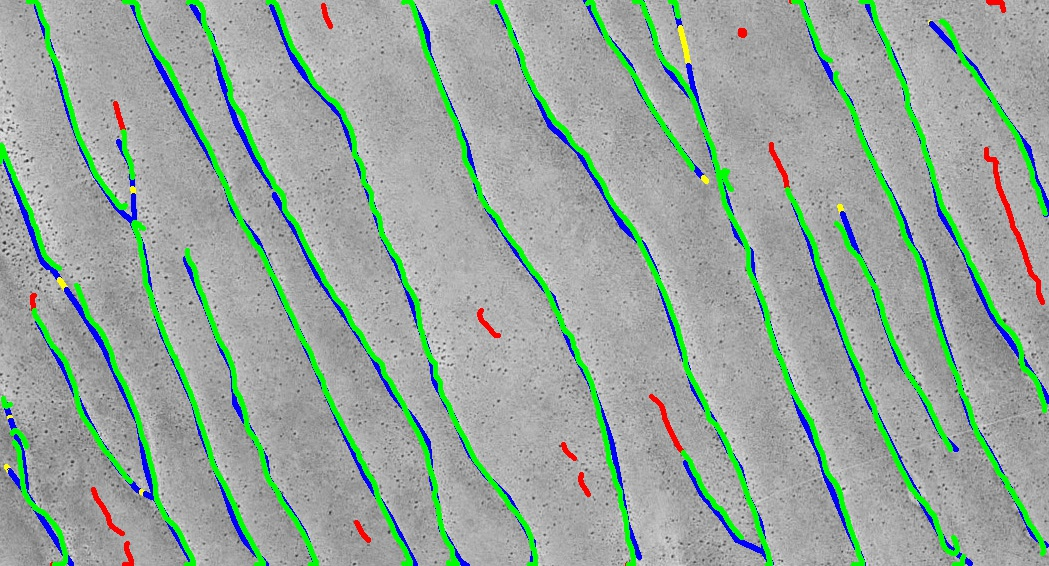
\includegraphics[width=1.0\linewidth]{figures/mixed_ml_grad_kalahari_results}
		\caption{ Kalahari Training }
		\label{fig:mixed_ml_grad_kalahari_results}
	\end{subfigure}
	\begin{subfigure}{0.48\textwidth}
		\centering
		%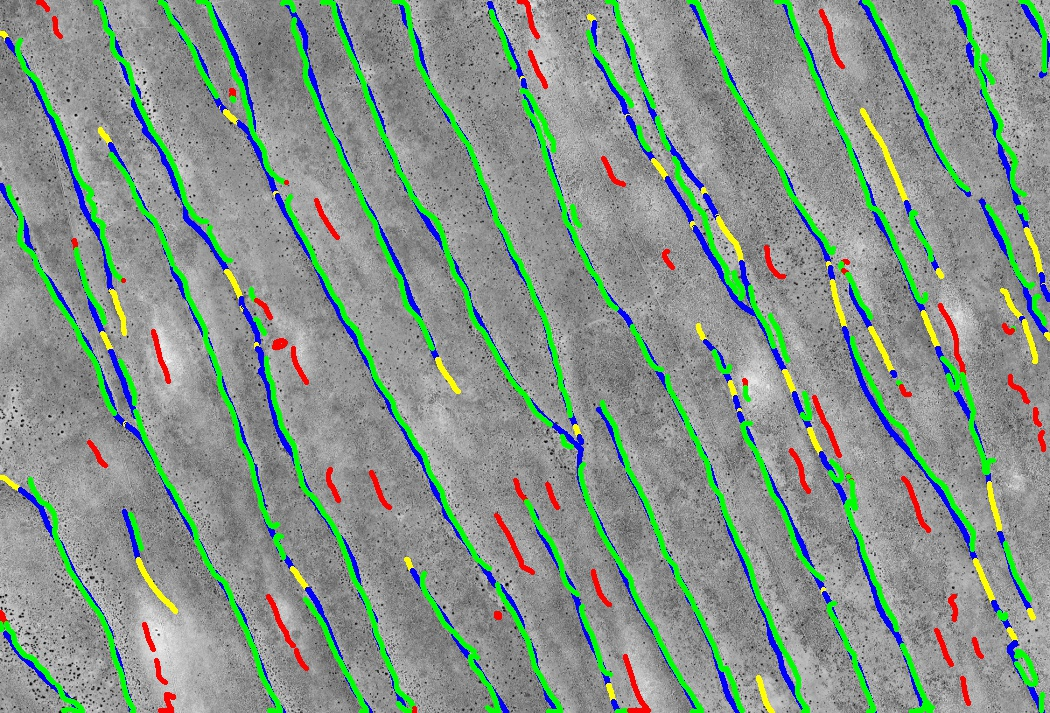
\includegraphics[width=1.0\linewidth]{figures/mixed_ml_grad_kalahari_test_results}
		\caption{ Kalahari Test }
		\label{fig:mixed_ml_grad_kalahari_test_results}
	\end{subfigure}
	\begin{subfigure}{0.48\textwidth}
		\centering
		%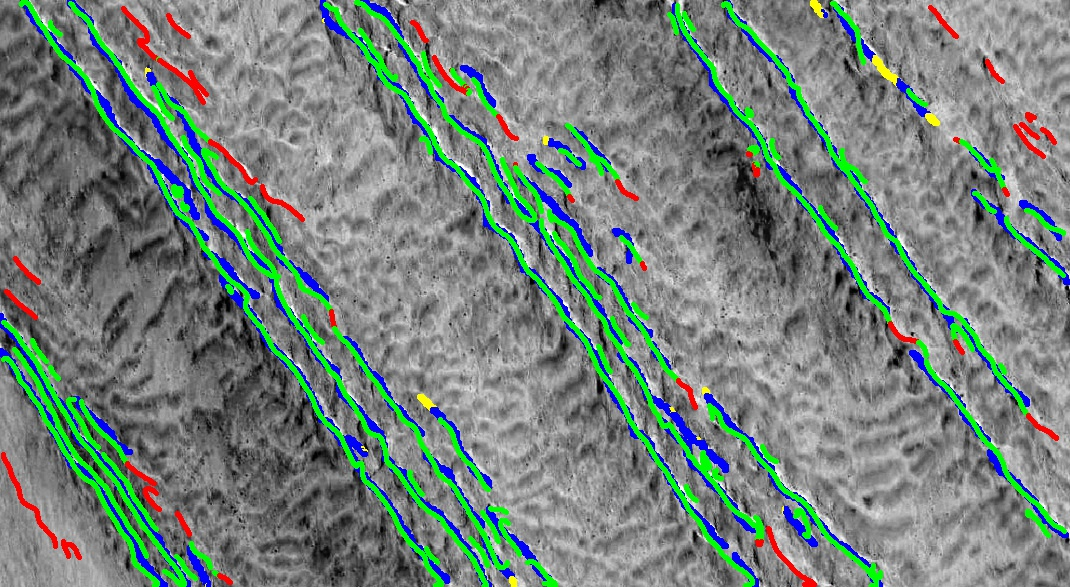
\includegraphics[width=1.0\linewidth]{figures/mixed_ml_grad_namib_results}
		\caption{ Namib Training }
		\label{fig:mixed_ml_grad_namib_results}
	\end{subfigure}
	\begin{subfigure}{0.48\textwidth}
		\centering
		%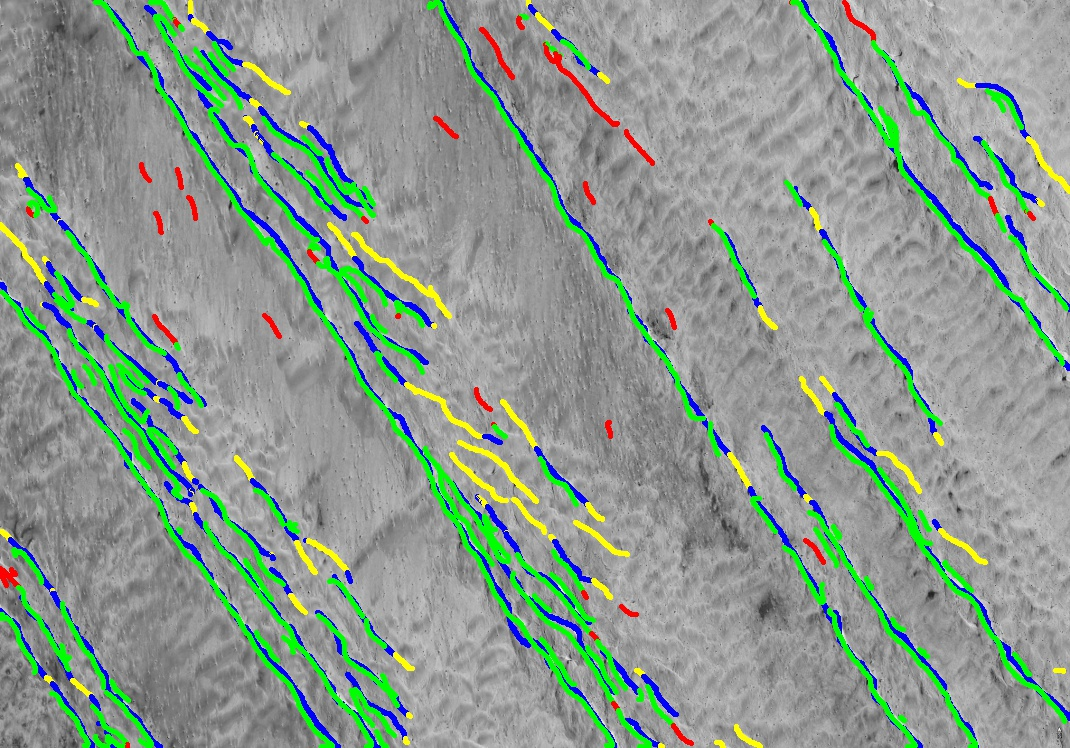
\includegraphics[width=1.0\linewidth]{figures/mixed_ml_grad_namib_test_results}
		\caption{ Namib Test }
		\label{fig:mixed_ml_grad_namib_test_results}
	\end{subfigure}
	\begin{subfigure}{0.48\textwidth}
		\centering
		%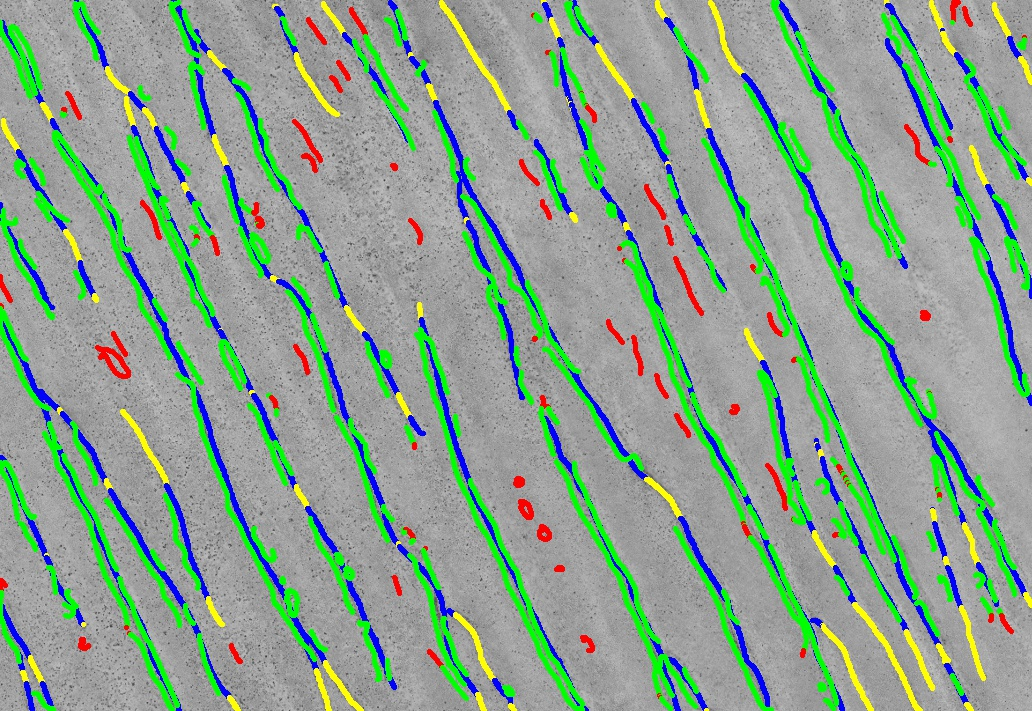
\includegraphics[width=1.0\linewidth]{figures/mixed_ml_grad_simpson_results}
		\caption{ Simpson Training }
		\label{fig:mixed_ml_grad_simpson_results}
	\end{subfigure}
	\begin{subfigure}{0.48\textwidth}
		\centering
		%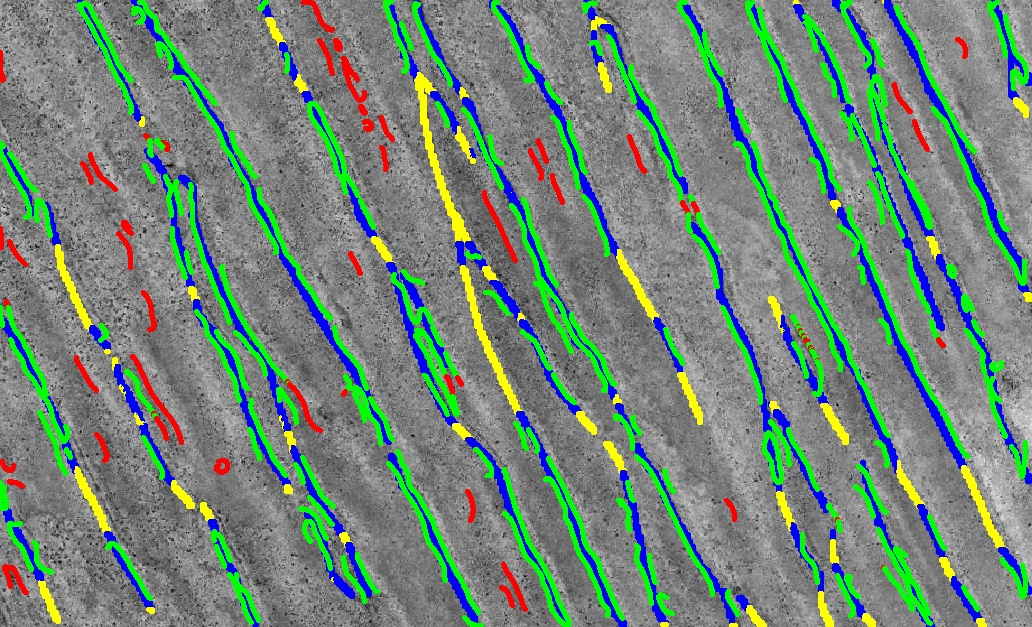
\includegraphics[width=1.0\linewidth]{figures/mixed_ml_grad_simpson_test_results}
		\caption{ Simpson Test }
		\label{fig:mixed_ml_grad_simpson_test_results}
	\end{subfigure}
\end{figure}
\begin{figure}
	\ContinuedFloat
	\centering
	\begin{subfigure}{0.48\textwidth}
		\centering
		%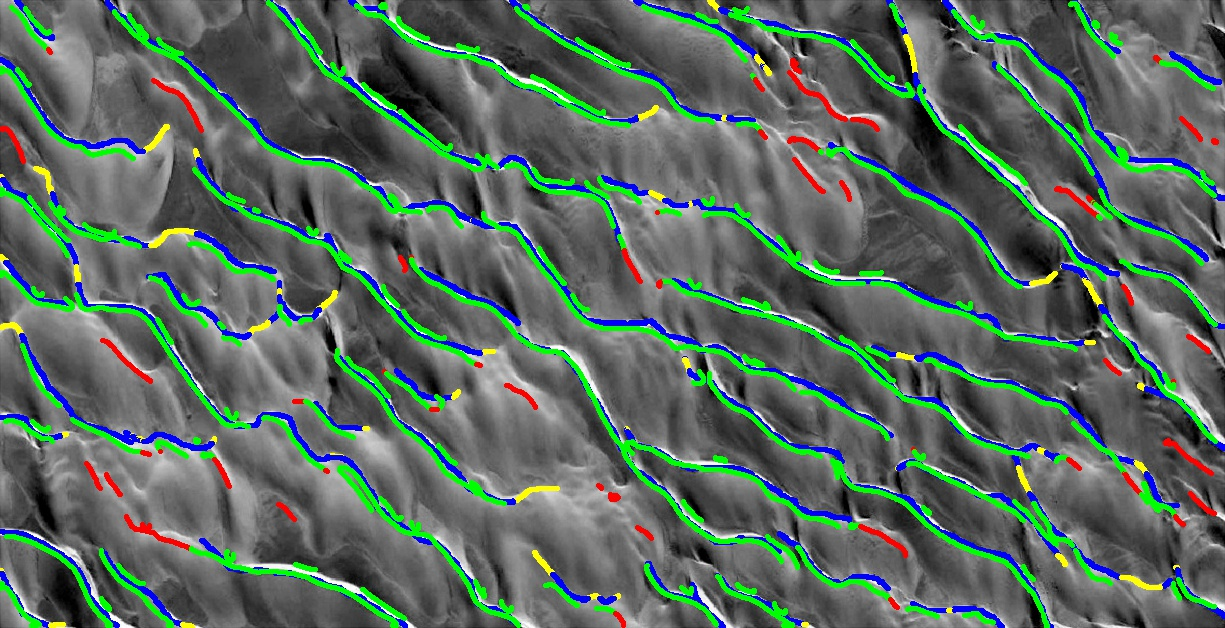
\includegraphics[width=1.0\linewidth]{figures/mixed_ml_grad_skeleton_coast_results}
		\caption{ Skeleton Coast Training }
		\label{fig:mixed_ml_grad_skeleton_coast_results}
	\end{subfigure}
	\begin{subfigure}{0.48\textwidth}
		\centering
		%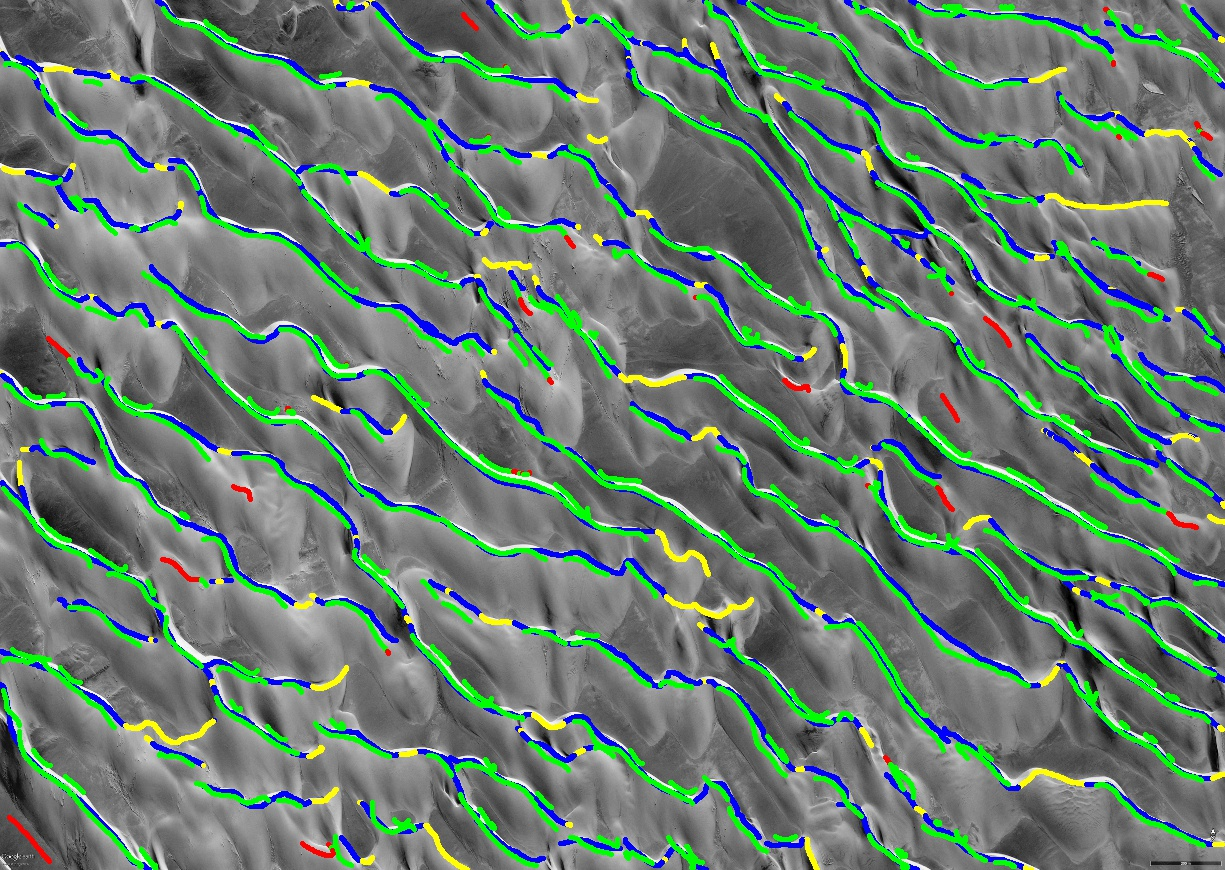
\includegraphics[width=1.0\linewidth]{figures/mixed_ml_grad_skeleton_coast_test_results}
		\caption{ Skeleton Coast Test }
		\label{fig:mixed_ml_grad_skeleton_coast_test_results}
	\end{subfigure}
	\begin{subfigure}{0.48\textwidth}
		\centering
		%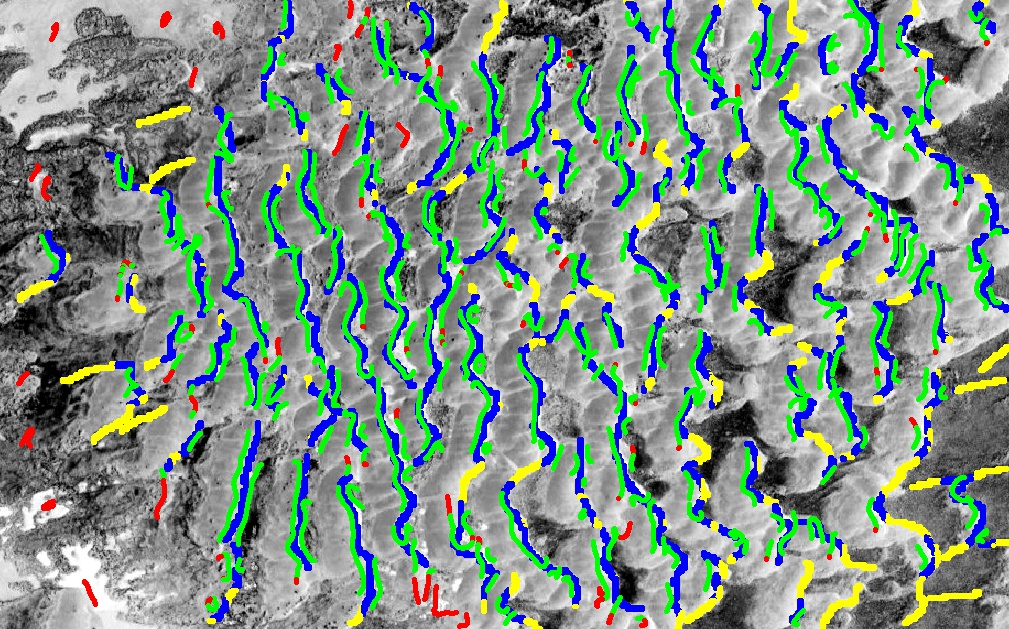
\includegraphics[width=1.0\linewidth]{figures/mixed_ml_grad_wdc_results}
		\caption{ WDC Training }
		\label{fig:mixed_ml_grad_wdc_results}
	\end{subfigure}
	\begin{subfigure}{0.48\textwidth}
		\centering
		%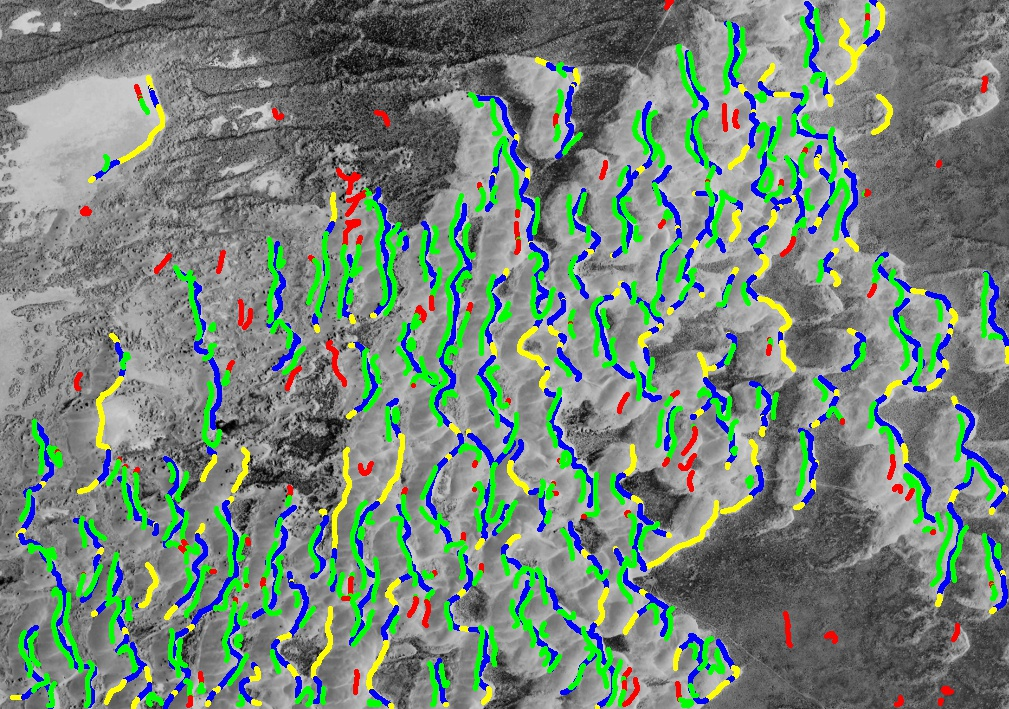
\includegraphics[width=1.0\linewidth]{figures/mixed_ml_grad_wdc_test_results}
		\caption{ WDC Test }
		\label{fig:mixed_ml_grad_wdc_test_results}
	\end{subfigure}
	\begin{subfigure}{0.48\textwidth}
		\centering
		%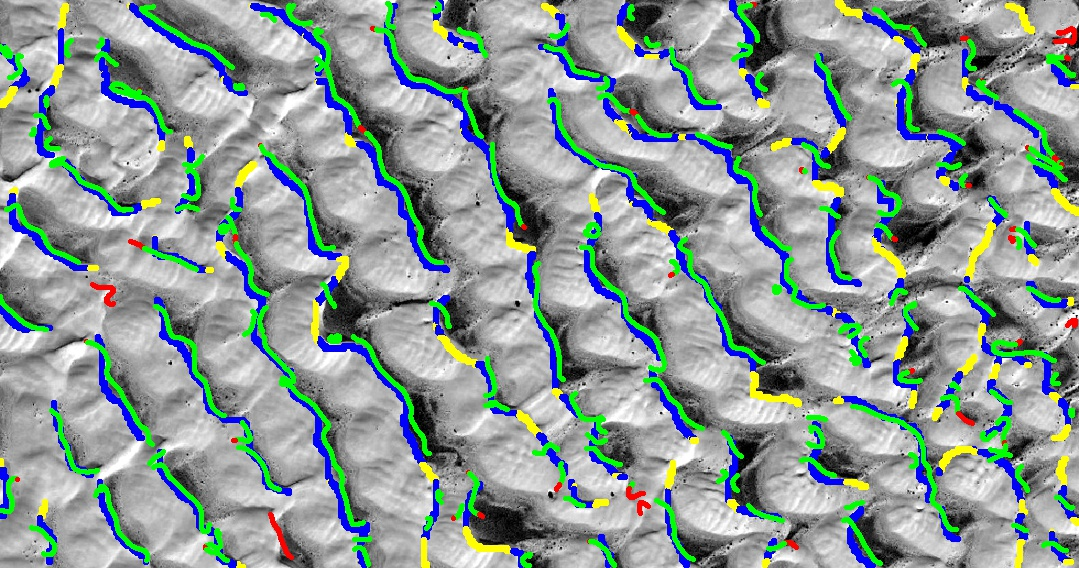
\includegraphics[width=1.0\linewidth]{figures/mixed_ml_grad_white_sands_results}
		\caption{ White Sands Training }
		\label{fig:mixed_ml_grad_white_sands_results}
	\end{subfigure}
	\begin{subfigure}{0.48\textwidth}
		\centering
		%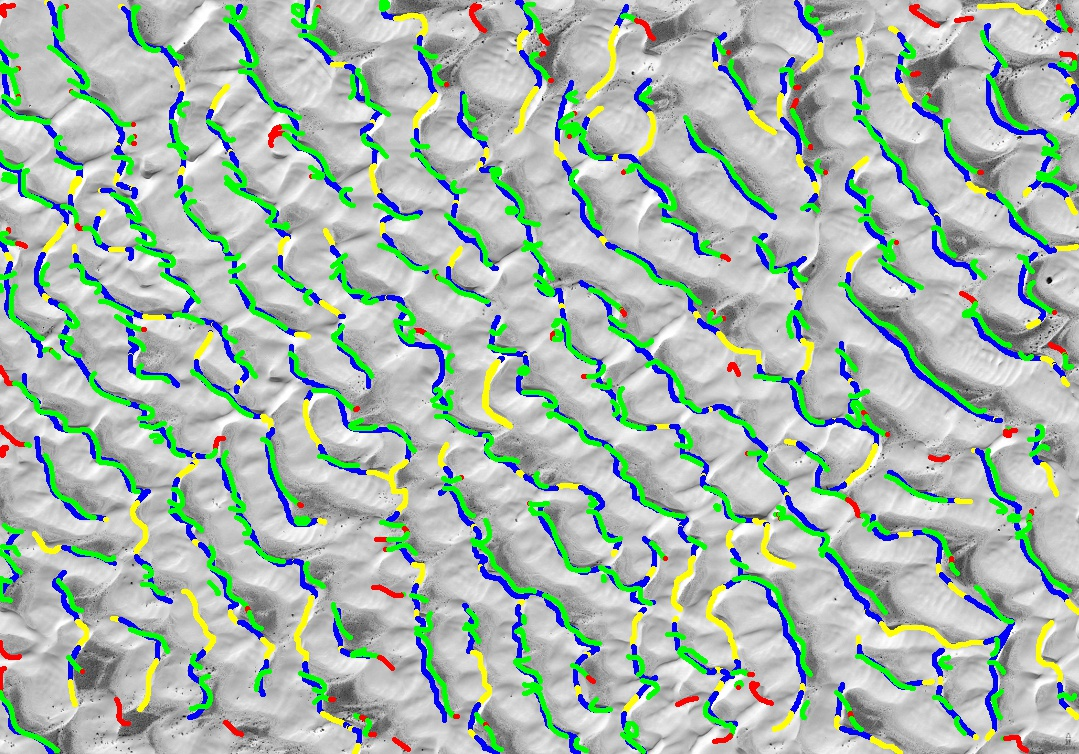
\includegraphics[width=1.0\linewidth]{figures/mixed_ml_grad_white_sands_test_results}
		\caption{ White Sands Test }
		\label{fig:mixed_ml_grad_white_sands_test_results}
	\end{subfigure}
	\caption{ The results of the crest-line detection for the mixed machine learning and gradient approach on terrestrial dataset for both the training images \subref{fig:ml_kalahari_results}, \subref{fig:ml_namib_results}, \subref{fig:ml_simpson_results}, \subref{fig:ml_skeleton_coast_results}, \subref{fig:ml_wdc_results}, \subref{fig:ml_white_sands_results}, and the test images \subref{fig:ml_kalahari_test_results}, \subref{fig:ml_namib_test_results}, \subref{fig:ml_simpson_test_results}, \subref{fig:ml_skeleton_coast_test_results}, \subref{fig:ml_wdc_test_results}, \subref{fig:ml_white_sands_test_results} using the GBT classifier and SIFT features. \underline{\textbf{Legend}}: \emph{Green} - True Positives, \emph{Red} - False Positives, \emph{Yellow} - False Negatives, \emph{Blue} - Ground truth correctly detected. }
	\label{fig:mixed_ml_grad_results}
\end{figure}

The results shown are an overall improvement on the machine learning method itself, notably an increased precision. Combining the machine learning and gradient orientation approaches results in many less false positives while preserving similar recall rates as shown in Tables \ref{tab:ml_grad_PR} and \ref{tab:cross_region_ml_grad_approach_results}. The metrics measured shown in Tables \ref{tab:ml_grad_metrics_error} and \ref{tab:cross_region_ml_grad_metrics_error} are similar to the standard machine learning approach. Unfortunately, there are no improvements for the cross region machine learning models. The method still struggles with more complex dune patterns, especially the White Sands region, shown in Figures \ref{fig:mixed_ml_grad_white_sands_results} and \ref{fig:mixed_ml_grad_white_sands_test_results}.

The method was also tested on another dataset. The Mars dataset, described in section \ref{subsec:mars_dataset} was constructed and used in the research presented in \cite{vaz_object_based_dune_analysis}. The results presented in this paper were acquired and the same evaluation methodology was applied on their results. We ran our method on the dataset, therefore we can compare the results side-by-side.

The region was sub-sampled into sixteen sub-region for efficient processing. The machine learning method requires a training set, therefore, half of the regions where used for training and the remaining half for testing. For simplicity, odd regions were used for training and even for testing. The precision/recall and dune metrics results for both the Vaz and our method are presented in Tables \ref{tab:ml_grad_mars_results} and \ref{tab:ml_grad_metrics_error}.

\begin{table}
	\centering
	\caption{ Precision and Recall results of the mixed machine learning and gradient-based method presented in section \ref{subsec:mixed_ml_gradient_approach} (GBT-SIFT) trained on the Mars dataset presented in \ref{subsec:mars_dataset}, compared to the results in \cite{vaz_object_based_dune_analysis}. Shown are the results of both the training set (odd areas) in (a), and test set (even areas) in (b). }
	\label{tab:ml_grad_mars_results}
	\begin{subtable}{0.98\textwidth}
		\centering
		\begin{tabu} to 0.9\textwidth { | X[2,c] || X[1,c] | X[1,c] || X[1,c] | X[1,c] | }
			\hline
			\multirow{2}{*}{\textbf{Sub-Regions}} & \multicolumn{2}{c||}{\textbf{Vaz \cite{vaz_object_based_dune_analysis} Results}} &  \multicolumn{2}{c|}{\textbf{Our Results}} \\
			\cline{2-5}
			& \textbf{Precision} & \textbf{Recall} & \textbf{Precision} & \textbf{Recall} \\
			\hline
			Area 1 & 0.4256 & 0.8454 & \textbf{0.6532} & \textbf{0.8563} \\
			Area 3 & 0.4725 & 0.9770 & \textbf{0.7367} & 0.9102 \\
			Area 5 & 0.5145 & 0.9067 & \textbf{0.7147} & 0.8346 \\
			Area 7 & 0.3055 & 0.9618 & \textbf{0.5496} & 0.9213 \\
			Area 9 & 0.3904 & 0.9126 & 0.3751 & \textbf{0.9486} \\
			Area 11 & 0.2491 & 0.7691 & 0.2151 & \textbf{0.9053} \\
			Area 13 & 0.3436 & 0.7702 & \textbf{0.3573} & \textbf{0.8489} \\
			\hline
		\end{tabu}
		\caption{Precision Recall Training Region Results: Vaz \cite{vaz_object_based_dune_analysis} vs Our Approach }
		\label{tab:ml_grad_mars_training_results}
	\end{subtable}
	\begin{subtable}{0.98\textwidth}
		\centering
		\begin{tabu} to 0.9\textwidth { | X[2,c] || X[1,c] | X[1,c] || X[1,c] | X[1,c] | }
			\hline
			\multirow{2}{*}{\textbf{Sub-Regions}} & \multicolumn{2}{c||}{\textbf{Vaz \cite{vaz_object_based_dune_analysis} Results}} &  \multicolumn{2}{c|}{\textbf{Our Results}} \\
			\cline{2-5}
			& \textbf{Precision} & \textbf{Recall} & \textbf{Precision} & \textbf{Recall} \\
			\hline
			Area 2 & 0.4451 & 0.8538 & \textbf{0.7823} & \textbf{0.9001} \\
			Area 4 & 0.4521 & 0.8750 & \textbf{0.7189} & 0.8274 \\
			Area 6 & 0.4516 & 0.9126 & 0.3564 & 0.4792 \\
			Area 8 & 0.4330 & 0.8518 & \textbf{0.6726} & 0.7991 \\
			Area 10 & 0.4541 & 0.8463 & \textbf{0.5259} & \textbf{0.8618} \\
			Area 12 & 0.4140 & 0.8736 & \textbf{0.4374} & \textbf{0.9043} \\
			Area 15 & 0.1404 & 0.9449 & 0.0880 & 0.2777 \\
			\hline
		\end{tabu}
		\caption{Precision Recall Test Region Results: \cite{vaz_object_based_dune_analysis} vs Our Approach }
		\label{tab:ml_grad_mars_test_results}
	\end{subtable}
\end{table}

\begin{table}
	\centering
	\caption{ Dune metrics results of the mixed machine learning and gradient-based method on the Mars dataset presented in \ref{subsec:mars_dataset}. The dune metrics were comuted on our crest-line detection results, the ground truth, and the crest-lines detected in \cite{vaz_object_based_dune_analysis}. Shown are the results of both the training set (odd areas) in (a), and test set (even areas) in (b). }
	\label{tab:ml_grad_mars_metrics_error}
	\begin{subtable}{0.98\textwidth}
		\centering
		\begin{tabu} to 0.9\textwidth { | X[2,c] || X[1,c] | X[1,c] || X[1,c] | X[1,c] | }
			\hline
			\multirow{2}{*}{\textbf{Sub-Regions}} & \multicolumn{2}{c||}{\textbf{Vaz \cite{vaz_object_based_dune_analysis} Results}} &  \multicolumn{2}{c|}{\textbf{Our Results}} \\
			\cline{2-5}
			& \textbf{$\Delta_{\theta}$} & \textbf{$\Delta_{d}$ (Pixels)} & \textbf{$\Delta_{\theta}$} & \textbf{$\Delta_{d}$ (Pixels)} \\
			\hline
			Area 1 & 5.0668\textdegree & 40.6086 & \textbf{1.6556\textdegree} & \textbf{12.748} \\
			Area 3 & 5.5938\textdegree & 52.1585 & \textbf{2.3637\textdegree} & \textbf{7.4039} \\
			Area 5 & 8.12824\textdegree & 93.7826 & \textbf{2.0505\textdegree} & \textbf{4.8174} \\
			Area 7 & 6.39212\textdegree & 28.3885 & \textbf{2.5625\textdegree} & \textbf{10.6288} \\
			Area 9 & 5.5570\textdegree & 74.2544 & 9.8787\textdegree & \textbf{8.1765} \\
			Area 11 & 22.1351\textdegree & 40.2464 & \textbf{3.3544\textdegree} & \textbf{8.9837} \\
			Area 13 & 20.5087\textdegree & 89.5503 & \textbf{14.651\textdegree} & \textbf{9.7079} \\
			\hline
		\end{tabu}
		\caption{Computed Dune Metrics Results (Training Regions): Vaz \cite{vaz_object_based_dune_analysis} vs Our Approach }
		\label{ tab:ml_grad_mars_training_metrics_error }
	\end{subtable}
	\begin{subtable}{0.98\textwidth}
		\centering
		\begin{tabu} to 0.9\textwidth { | X[2,c] || X[1,c] | X[1,c] || X[1,c] | X[1,c] | }
			\hline
			\multirow{2}{*}{\textbf{Sub-Regions}} & \multicolumn{2}{c||}{\textbf{Vaz \cite{vaz_object_based_dune_analysis} Results}} &  \multicolumn{2}{c|}{\textbf{Our Results}} \\
			\cline{2-5}
			& \textbf{$\Delta_{\theta}$} & \textbf{$\Delta_{d}$ (Pixels)} & \textbf{$\Delta_{\theta}$} & \textbf{$\Delta_{d}$ (Pixels)} \\
			\hline
			Area 2 & 5.5938\textdegree & 52.1585 & 5.8210\textdegree & \textbf{35.053} \\
			Area 4 & 6.3921\textdegree & 28.3885 & \textbf{1.9697\textdegree} & \textbf{21.4148} \\
			Area 6 & 2.51432\textdegree & 12.6348 & 9.0910\textdegree & 17.5553 \\
			Area 8 & 1.7801\textdegree & 35.8738 & 3.4364\textdegree & \textbf{5.8379} \\
			Area 10 & 1.7096\textdegree & 54.185 & 2.6398\textdegree & \textbf{6.9980} \\
			Area 12 & 8.3404\textdegree & 63.7937 & \textbf{2.0865\textdegree} & \textbf{46.1008} \\
			Area 15 & 17.1538\textdegree & 0.9386 & \textbf{11.7136\textdegree} & 55.664 \\
			\hline
		\end{tabu}
		\caption{Computed Dune Metrics Results (Test Regions): \cite{vaz_object_based_dune_analysis} vs Our Approach }
		\label{tab:ml_grad_mars_test_metrics_error}
	\end{subtable}
\end{table}

Clearly, the results show that the performance of our method is superior, mainly in precision. Recall values are roughly equivalent in most areas, but our precision is typically much better. This can be attributed to the improved localization of the crest-lines using the response maps. There are a few cases in which our method fails to deliver high precision and recall. These cases can be easily explained simply by examining the projected results in Figure \ref{fig:mixed_ml_grad_mars_results}.

\begin{figure}
	\centering
	\begin{subfigure}{\textwidth}
		\centering
		%\includegraphics[width=0.48\linewidth]{figures/Area_1_vaz_results_}
		%\includegraphics[width=0.48\linewidth]{figures/Area_1_results_}
		\caption{ Area 1: Vaz \cite{vaz_object_based_dune_analysis} and Our Results }
		\label{fig:mixed_ml_grad_area1_results}
	\end{subfigure}
	\begin{subfigure}{\textwidth}
		\centering
		%\includegraphics[width=0.48\linewidth]{figures/Area_2_vaz_results_}
		%\includegraphics[width=0.48\linewidth]{figures/Area_2_results_}
		\caption{ Area 2: Vaz \cite{vaz_object_based_dune_analysis} and Our Results }
		\label{fig:mixed_ml_grad_area2_results}
	\end{subfigure}
	\begin{subfigure}{\textwidth}
		\centering
		%\includegraphics[width=0.48\linewidth]{figures/Area_3_vaz_results_}
		%\includegraphics[width=0.48\linewidth]{figures/Area_3_results_}
		\caption{ Area 3: Vaz \cite{vaz_object_based_dune_analysis} and Our Results }
		\label{fig:mixed_ml_grad_area3_results}
	\end{subfigure}
	\begin{subfigure}{\textwidth}
		\centering
		%\includegraphics[width=0.48\linewidth]{figures/Area_4_vaz_results_}
		%\includegraphics[width=0.48\linewidth]{figures/Area_4_results_}
		\caption{ Area 4: Vaz \cite{vaz_object_based_dune_analysis} and Our Results }
		\label{fig:mixed_ml_grad_area4_results}
	\end{subfigure}
	\begin{subfigure}{\textwidth}
		\centering
		%\includegraphics[width=0.48\linewidth]{figures/Area_5_vaz_results_}
		%\includegraphics[width=0.48\linewidth]{figures/Area_5_results_}
		\caption{ Area 5: Vaz \cite{vaz_object_based_dune_analysis} and Our Results }
		\label{fig:mixed_ml_grad_area5_results}
	\end{subfigure}
\end{figure}
\begin{figure}
	\ContinuedFloat
	\centering
	\begin{subfigure}{\textwidth}
		\centering
		%\includegraphics[width=0.48\linewidth]{figures/Area_6_vaz_results_}
		%\includegraphics[width=0.48\linewidth]{figures/Area_6_results_}
		\caption{ Area 6: Vaz \cite{vaz_object_based_dune_analysis} and Our Results }
		\label{fig:mixed_ml_grad_area6_results}
	\end{subfigure}
	\begin{subfigure}{\textwidth}
		\centering
		%\includegraphics[width=0.48\linewidth]{figures/Area_7_vaz_results_}
		%\includegraphics[width=0.48\linewidth]{figures/Area_7_results_}
		\caption{ Area 7: Vaz \cite{vaz_object_based_dune_analysis} and Our Results }
		\label{fig:mixed_ml_grad_area7_results}
	\end{subfigure}
	\begin{subfigure}{\textwidth}
		\centering
		%\includegraphics[width=0.48\linewidth]{figures/Area_8_vaz_results_}
		%\includegraphics[width=0.48\linewidth]{figures/Area_8_results_}
		\caption{ Area 8: Vaz \cite{vaz_object_based_dune_analysis} and Our Results }
		\label{fig:mixed_ml_grad_area8_results}
	\end{subfigure}
	\begin{subfigure}{\textwidth}
		\centering
		%\includegraphics[width=0.48\linewidth]{figures/Area_9_vaz_results_}
		%\includegraphics[width=0.48\linewidth]{figures/Area_9_results_}
		\caption{ Area 9: Vaz \cite{vaz_object_based_dune_analysis} and Our Results }
		\label{fig:mixed_ml_grad_area9_results}
	\end{subfigure}
	\begin{subfigure}{\textwidth}
		\centering
		%\includegraphics[width=0.48\linewidth]{figures/Area_10_vaz_results_}
		%\includegraphics[width=0.48\linewidth]{figures/Area_10_results_}
		\caption{ Area 10: Vaz \cite{vaz_object_based_dune_analysis} and Our Results }
		\label{fig:mixed_ml_grad_area10_results}
	\end{subfigure}
\end{figure}
\begin{figure}
	\ContinuedFloat
	\centering
	\begin{subfigure}{\textwidth}
		\centering
		%\includegraphics[width=0.48\linewidth]{figures/Area_11_vaz_results_}
		%\includegraphics[width=0.48\linewidth]{figures/Area_11_results_}
		\caption{ Area 11: Vaz \cite{vaz_object_based_dune_analysis} and Our Results }
		\label{fig:mixed_ml_grad_area11_results}
	\end{subfigure}
	\begin{subfigure}{\textwidth}
		\centering
		%\includegraphics[width=0.48\linewidth]{figures/Area_12_vaz_results_}
		%\includegraphics[width=0.48\linewidth]{figures/Area_12_results_}
		\caption{ Area 12: Vaz \cite{vaz_object_based_dune_analysis} and Our Results }
		\label{fig:mixed_ml_grad_area12_results}
	\end{subfigure}
	\begin{subfigure}{\textwidth}
		\centering
		%\includegraphics[width=0.48\linewidth]{figures/Area_13_vaz_results_}
		%\includegraphics[width=0.48\linewidth]{figures/Area_13_results_}
		\caption{ Area 13: Vaz \cite{vaz_object_based_dune_analysis} and Our Results }
		\label{fig:mixed_ml_grad_area13_results}
	\end{subfigure}
	\begin{subfigure}{\textwidth}
		\centering
		%\includegraphics[width=0.48\linewidth]{figures/Area_15_vaz_results_}
		%\includegraphics[width=0.48\linewidth]{figures/Area_15_results_}
		\caption{ Area 15: Vaz \cite{vaz_object_based_dune_analysis} and Our Results }
		\label{fig:mixed_ml_grad_area15_results}
	\end{subfigure}
	\caption{ Crest-line detection results plotted for all regions used in the Mars dataset. The Vaz \cite{vaz_object_based_dune_analysis} results (on the left) compared to our results (on the right). \underline{\textbf{Legend}}: \emph{Green} - True Positives, \emph{Red} - False Positives, \emph{Yellow} - False Negatives, \emph{Blue} - Ground truth correctly detected. }
	\label{fig:mixed_ml_grad_mars_results}
\end{figure}

As with Figure \ref{fig:mixed_ml_grad_results}, the results shown in Figure \ref{fig:mixed_ml_grad_mars_results} display the detected crest-lines overlapped with the ground truth of each area. The color schemes shows green lines as correctly detected crest-lines and red lines as false positives. Blue lines are ground truth crest-lines which have been correctly identified, and yellow lines are unidentified ground truth crest-lines (false negatives). 

The first notable issue with the Vaz results are the noisiness and disjointness of the detections, while our results are much smoother, less noisy, contiguous segments. Also, in many cases, the Vaz results show duplicate parallel detections next to each crest-lines which falsely increase the apparent precision, while our results are more accurate single segments for each crest-lines. This especially noticeable in areas 1, 5, 6, 7 and 10 (Figures \ref{fig:mixed_ml_grad_area1_results}, \ref{fig:mixed_ml_grad_area5_results}, \ref{fig:mixed_ml_grad_area6_results}, \ref{fig:mixed_ml_grad_area7_results} and \ref{fig:mixed_ml_grad_area10_results}).

The final issue is the ground truth itself. The ground truth was labeled by the Vaz researchers and is for the most part accurate, but there are many discrepancies. In many cases, some crest-lines are missing from the ground truth, and often the localization of the ground truth itself is quite poor. Areas 9 and 15 (\ref{fig:mixed_ml_grad_area9_results}, \ref{fig:mixed_ml_grad_area15_results}) are good examples of poor labeling of crest-lines in the ground truth. Many of the detections in those areas should in fact be true positives. Area 6 (\ref{fig:mixed_ml_grad_area6_results}) is a good example of poor localization. Our results show that the actual crest-lines were detected but because the ground truth is offset from the actual crest-lines (by a distance greater than our error threshold $\epsilon$), the detections count as false positives when they really should be true positives. The effect of these issues are reflected in the results generated in Tables \ref{tab:ml_grad_mars_results} and \ref{tab:ml_grad_metrics_error}.

As stated previously, determining true positives was dependent on the selection of the distance error threshold parameter $\epsilon$. The parameter was admittedly arbitrary selected to be $\epsilon = 10$, based on what seems to be a reasonable allowable error in localization of crest-lines. The parameter $\epsilon$ directly affects the reported precision and recall results. In order to have a better understanding and a better comparison, the plots in Figure \ref{fig:precision_recall_vs_epsilon} show the precision and recall results versus the distance error threshold $\epsilon$ parameter, for both our approach and the Vaz results.

\begin{figure}
	\centering
	\begin{subfigure}{0.48\textwidth}
		\centering
		%\includegraphics[width=1.0\linewidth]{figures/area1_pr_epsilon}
		\caption{ Area 1: PR vs $\epsilon$}
		\label{fig:precision_recall_vs_epsilon_area1}
	\end{subfigure}
	\begin{subfigure}{0.48\textwidth}
		\centering
		%\includegraphics[width=1.0\linewidth]{figures/area2_pr_epsilon}
		\caption{ Area 2: PR vs $\epsilon$}
		\label{fig:precision_recall_vs_epsilon_area2}
	\end{subfigure}
	\caption{ Plots of the Precision and Recall comparison between our method and Vaz \cite{vaz_object_based_dune_analysis} for Area 1 (a) and Area (b) as the allowable distance threshold value $\epsilon$ increases. }
	\label{fig:precision_recall_vs_epsilon}
\end{figure}

In areas 1 and 2 (Figures \ref{fig:precision_recall_vs_epsilon_area1}, \ref{fig:precision_recall_vs_epsilon_area2}), the recall values stay roughly equivalent for both methods, with our approach slightly leading in area 1 and with the Vaz results having a slight edge in area 2. The reason for this is most likely because the machine learning method was trained on odd areas and tested on even areas, therefore, a lower recall should be expected. The main distinction in the two approaches is the precision results. Our approach offers vastly and consistently better precision than the Vaz approach.

To summarize the results, the machine learning approaches are by far the best methods for detecting the crest-lines. This is easily seen simply in the numbers, shown in Tables \ref{tab:machine_learning_approach_results} to \ref{tab:ml_grad_mars_metrics_error}. Not only are the precision, recall, and metrics results better in almost every case, the quality of the produced crest-lines are much better. The detected crest-lines in the machine learning methods are generally smoother and are more contiguous that the previous methods.

The main benefits of the machine learning is that it is a much simpler approach than other appearance based approach. By simpler, we mean that fewer parameters and optimization are required to achieve good results. In appearance based approaches presented in sections \ref{subsection:appearance_based_approach}, \ref{subsec:edge_based_detection}, \ref{subsec:watershed_transform_segmentation_approach}, \ref{subsec:frequency_domain_approach}, and \ref{subsec:gradient_orientation_based}, many parameters are required in order to tune the performance of crest-line detection. Typically, the parameters also require optimization based on the appearance, scale, and contrast in each region. These factors are solved in machine learning model which simply learns the distinctions of crest-lines versus non-crest-lines.

The benefits of the machine learning method come at a cost. Labeled data is required in order to train the models, which requires the crest-lines in an image region to be manually and accurately traced by an expert. The process of creating the ground truth for training can be tedious and error prone. Also, there seems to be some struggles when training a model across regions of different types of dunes. If the dunes of two different regions are similar, then a single model might be sufficient. However, when training a model on linear dunes for example, the results of using this model on a complex dune structure may not be optimal.

The final section summarizes and discusses the work done in this research, along with offering potential future work methods. 